\chapter{t-SNE} 

\label{Chapter8} 

\section{Introduction}

The load profiles can present big data in a way, that can enable users or algorithms to extract activation patterns.
The one thing they do not offer is a comparison between activation patterns.
One such example would be when checking how similar are certain usage patterns.
This could be usage patterns within a household, where we are looking for appliances that are used similarly,
or when observing multiple buildings how their consumption differs. 
To measure the similarity of activation profiles, the t-SNE algorithm will be used.

The clustering of load profiles was used many times before like it was already described in related work chapter \ref{Chapter3}.
We will be working with dimensionality reduction, where clusters are usually formed due to similar data, the following clustering publications are still worth mentioning.
We have seen that authors \cite{GERBEC2005}, \cite{Jeong2021} and \cite{Joana2012} have clustered regular one-dimensional load profiles, as well as with 2D image-based load profiling in publications published by \cite{Park2019}. 

The publication by \cite{sne_energ} compared various dimensionality reduction techniques for clustering and visualization of load profiles.
Their goal was to compare Principal Component Analysis, Isometric Feature Mapping, Sammon Mapping, Locally Linear Embedding and Stochastic Neighbor Embedding.
They used power daily load profiles from residential and industrial areas.
This publication was of the closest resemblance to our goals, that we were able to find. 

In all cases, work has been done with the power load profile, whereas in this case, we will try to find similarities between activation profiles using a t-SNE algorithm.
Most of the publications used single-time dimensions, whereas we will use two-time dimensions.

Although the use-cases were presented in-depth in chapter \ref{Chapter4}, it is worth mentioning one specific use case.

The increasing price of energy resources, could lead to over-saving and living in cool homes.
By using similarity metrics between profiles across different buildings, it would be possible to detect outliers when it comes to heating. 
With this approach, it would be possible to detect users, that are living in below-average cool homes and offer them cheaper plans. 


\section{Goals}

The chapter will demonstrate the application of previously unused load profiles,
and show the practical use case using a t-SNE neighboring algorithm.

Using this algorithm we will show how user data is related in high dimensional space.
For this, we will use per-building, per-appliance load profiles with many combinations, where
each one enables us a different view of load profiles. 

\section{Methodology}

\subsection{Load profiles}

\subsubsection{Weekly-daily load profile}

During testing, a weekly-daily load profile constructed from a month of data will be used.
Y-axis will present the days in a week and X-axis presents the hours in a day.
Days are labeled from 0 to 6, and hours from 0 to 23.
Since we are working with images, the origin is placed in the upper-left corner. 
This means that a pixel in the upper-left corner presents the first hour in a week,
this would be a Monday from midnight to one o'clock. 
The lower-right corner presents the last hour of a week.
Since there are roughly 4 weeks in each month, each pixel will present 4 samples. 

\begin{figure}[H]
	\centering
	\caption{"Weekly per-appliance load profile"}
	\includegraphics[width=0.7\textwidth]{../Figures/LPS/WM_weekly.png}
	\label{fig:WM_weekly_2}
\end{figure}

One such example of profiles that we will use, was already presented in chapter \ref{chapter6} with figure \ref{fig:WM_weekly}.
For practical reasons, we are presenting it again here with figure \ref{fig:WM_weekly_2}.

\subsubsection{Bag of appliances load profile}

Another load profile that will be used at the end of the results section will be the bag-of-appliances load profile.
The profile was presented and analyzed in depth in chapter \ref{chapter6} and was presented in figure \ref{fig:BOA}.
But again, for ease-of-use purposes, we will summarize the profile here.

\begin{figure}[H]
	\centering
	\caption{"Universal presentation of per-building per-appliance load profile"}
	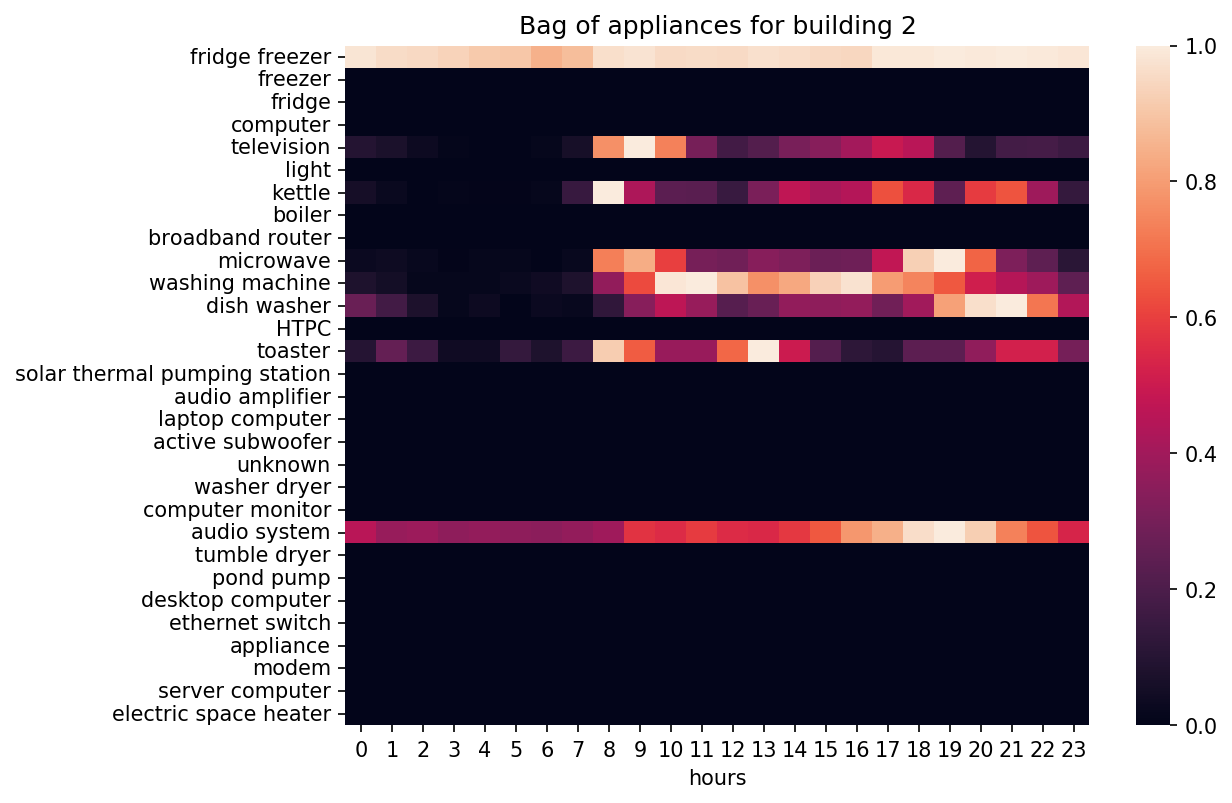
\includegraphics[width=1\textwidth]{../Figures/LPS/BOA.png}
	\label{fig:BOA2}
\end{figure}

To build the profile seen in figure \ref{fig:BOA2}, we used the data from all 5 datasets and made a list of the most commonly used appliances.
Only the top 30 appliances were selected.
This enables us to have the same load profile for all buildings, and thus enables us to see how the usage differs across them.
One problem that arises here is the missing appliances.
These appliances present themselves as a black line.
A lot of missing appliances may cause the image to be primarily black,
which could cause troubles for the algorithm processing this as an image.

\subsubsection{Samples}

We have on average roughly one year of data per building. 
In some cases few weeks and some up to 5 years for some appliances.
By slicing this data into 1-month long intervals and converting them to load profiles we were able to obtain 5218 samples.

\subsection{Datasets}

To present the results REFIT (\cite{REFIT}), UK-DALE  (\cite{UKDALE}), ECO  (\cite{ECO}), REDD  (\cite{REDD}) and iAWE  (\cite{iAWE}) datasets will be used.
Combined datasets include data for over 25 homes, where some have up to 5 years of data. 
The structure of datasets will be analyzed in larger depth in the next chapter \ref{Chapter7}. 

\subsection{t-SNE algorithm}

The t-SNE \cite{tsne2} or t-distribution stochastic neighboring embedding is a method for portraying high dimensional 
data in low dimensional space. This process is also known as dimensionality reduction.

One of the well-known dimensionality reduction algorithms is PCA.
The key difference between the two is that one is linear, and the other is non-linear.
PCA, linear, projects data in new space and finds the one with the least variance between data points.
SNE \cite{sne1}, non-linear, is composed of two main parts. The first one is 
converting the high-dimensional Euclidean distances between data points into conditional probabilities that represent similarities. \cite{sne1}
The pairs with high similarity have a high probability, and pairs with lower a low probability.
Second, it uses Kullback-Leibler divergence to minimize it with respect to a location on a map.
To achieve this it uses gradient descent to minimize the cost function.
Over many iterations, similar data points should be close together and far away from dissimilar objects.
Similar data points usually form clusters.

t-SNE uses SNE as a basis, except that it uses t-student distribution instead of normal to calculate the similarity.

In our case, two dimensions will be used. Since this is non-linear dimensionality reduction,
the axis usually presents dimensions that are hard to comprehend by the brain. 
Since the algorithm uses similarity at the base of the algorithm, it is possible to 
see which samples are more similar to each other.


\section{Results}

The results will be presented in three subsections, these are

\begin{itemize}
	\item Per-building load profile
	\item Per-appliance load profile
	\item Per-building per-appliance load profile
\end{itemize}

Most of the focus will be done on the per-appliance load profile since it is the most universal.

\subsection{Results for per-building load profiles}
\label{ssec:res_pb_lp}
This load profile is useful when it comes to comparing how 
activation patterns change over buildings and datasets.
Per-building data uses combined activations of all appliances to present 
the aggregated usage pattern. 

Figure \ref{fig:tsne_scatter_non_norm_all} is using non-normalized data, meaning
the number of appliances in a building will affect the end load profile.
The algorithm could pick up on how many appliances are being used.
In some cases, such as energy poverty detection, this information is useful, 
again in others we would like to find a more complex usage pattern.

\begin{figure}[H]
	\centering
	\caption{"Projection of per-building load profiles"}
	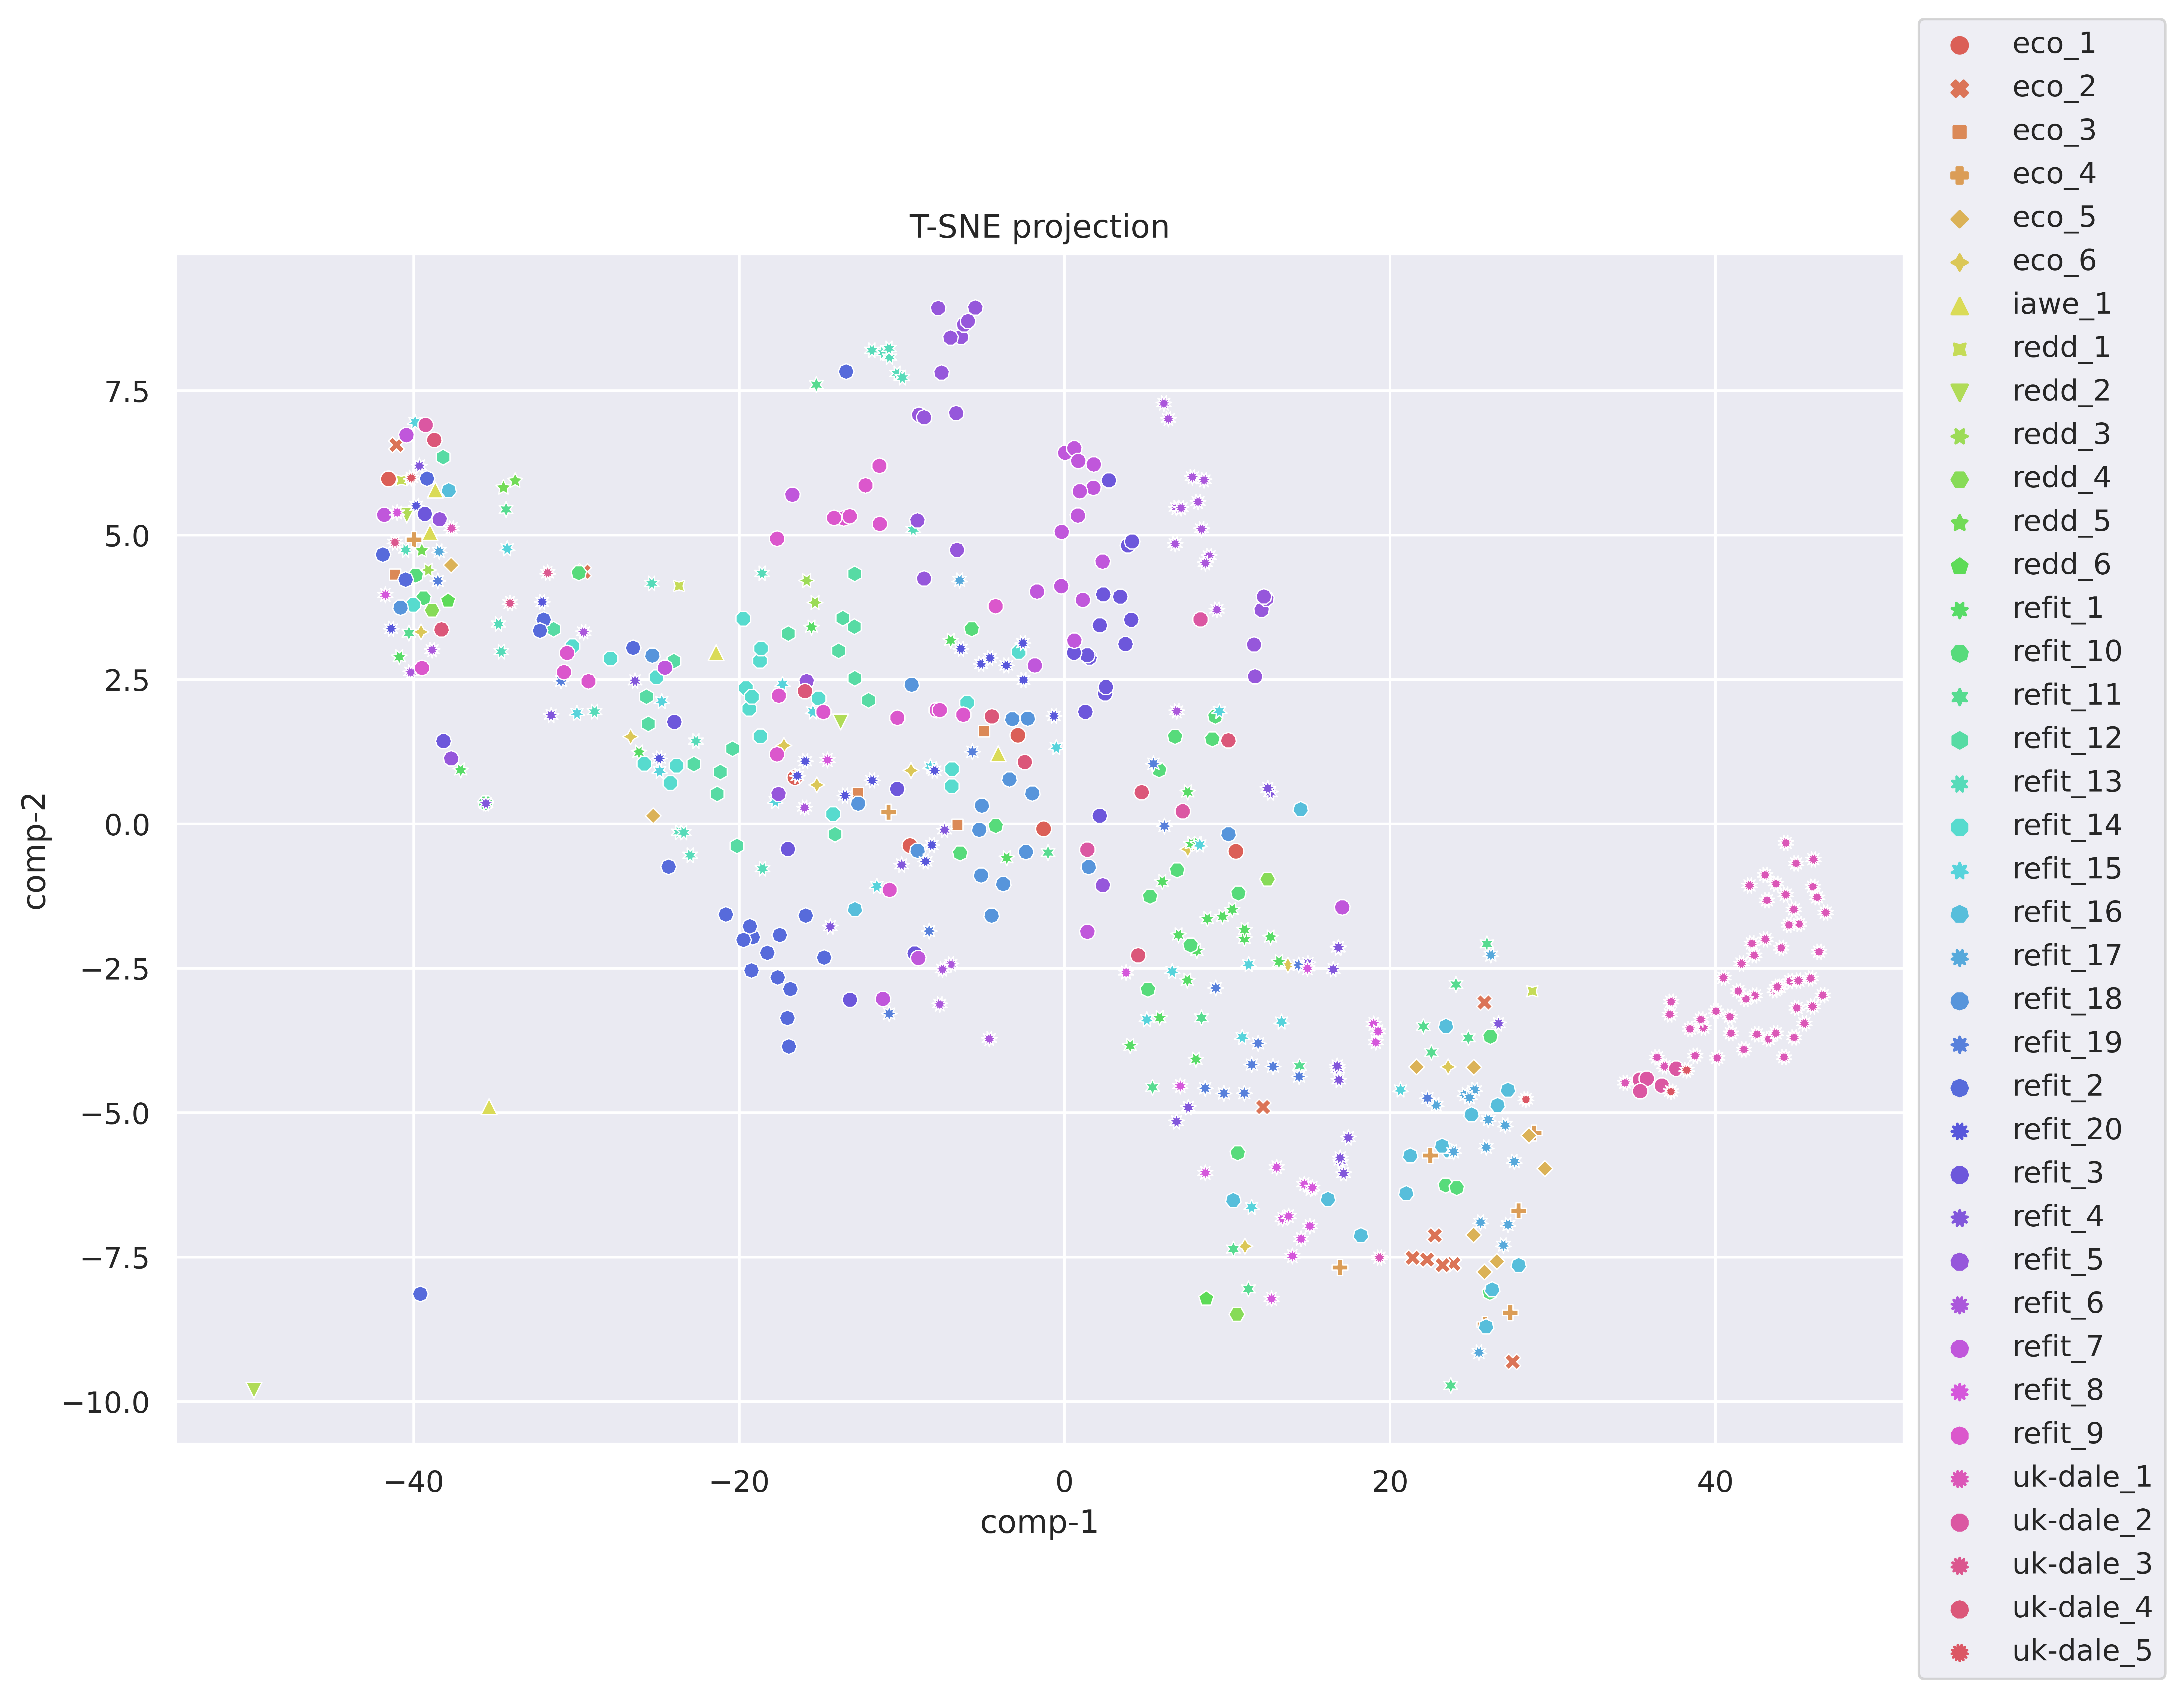
\includegraphics[width=1.2\textwidth]{Figures/TSNE/TSNE_per_building/non_norm/scatter_non_norm_all.png}
	\label{fig:tsne_scatter_non_norm_all}
\end{figure}

The figure \ref{fig:tsne_pb_img_scatter_allall} presents the actual load profile behind each sample. 
It is possible to see that on the left there are mostly samples with very little activity,
and on the left, we see samples with more activity.
Since the two plotted components are of a higher dimension, it is hard to guess what they present.
As said t-SNE gives us the intuition of how load profiles are connected in higher-dimensional space.

The following figures are best viewed in color and a digital format. 
Readers reading the digital version should have the ability to zoom into each cluster, and see the actual samples. 
Readers reading a paper version can still explore the high-resolution figures online via the provided link at the end of the document.

\begin{figure}[H]
	\centering
	\caption{"Projection of per-building load profiles with actual samples"}
	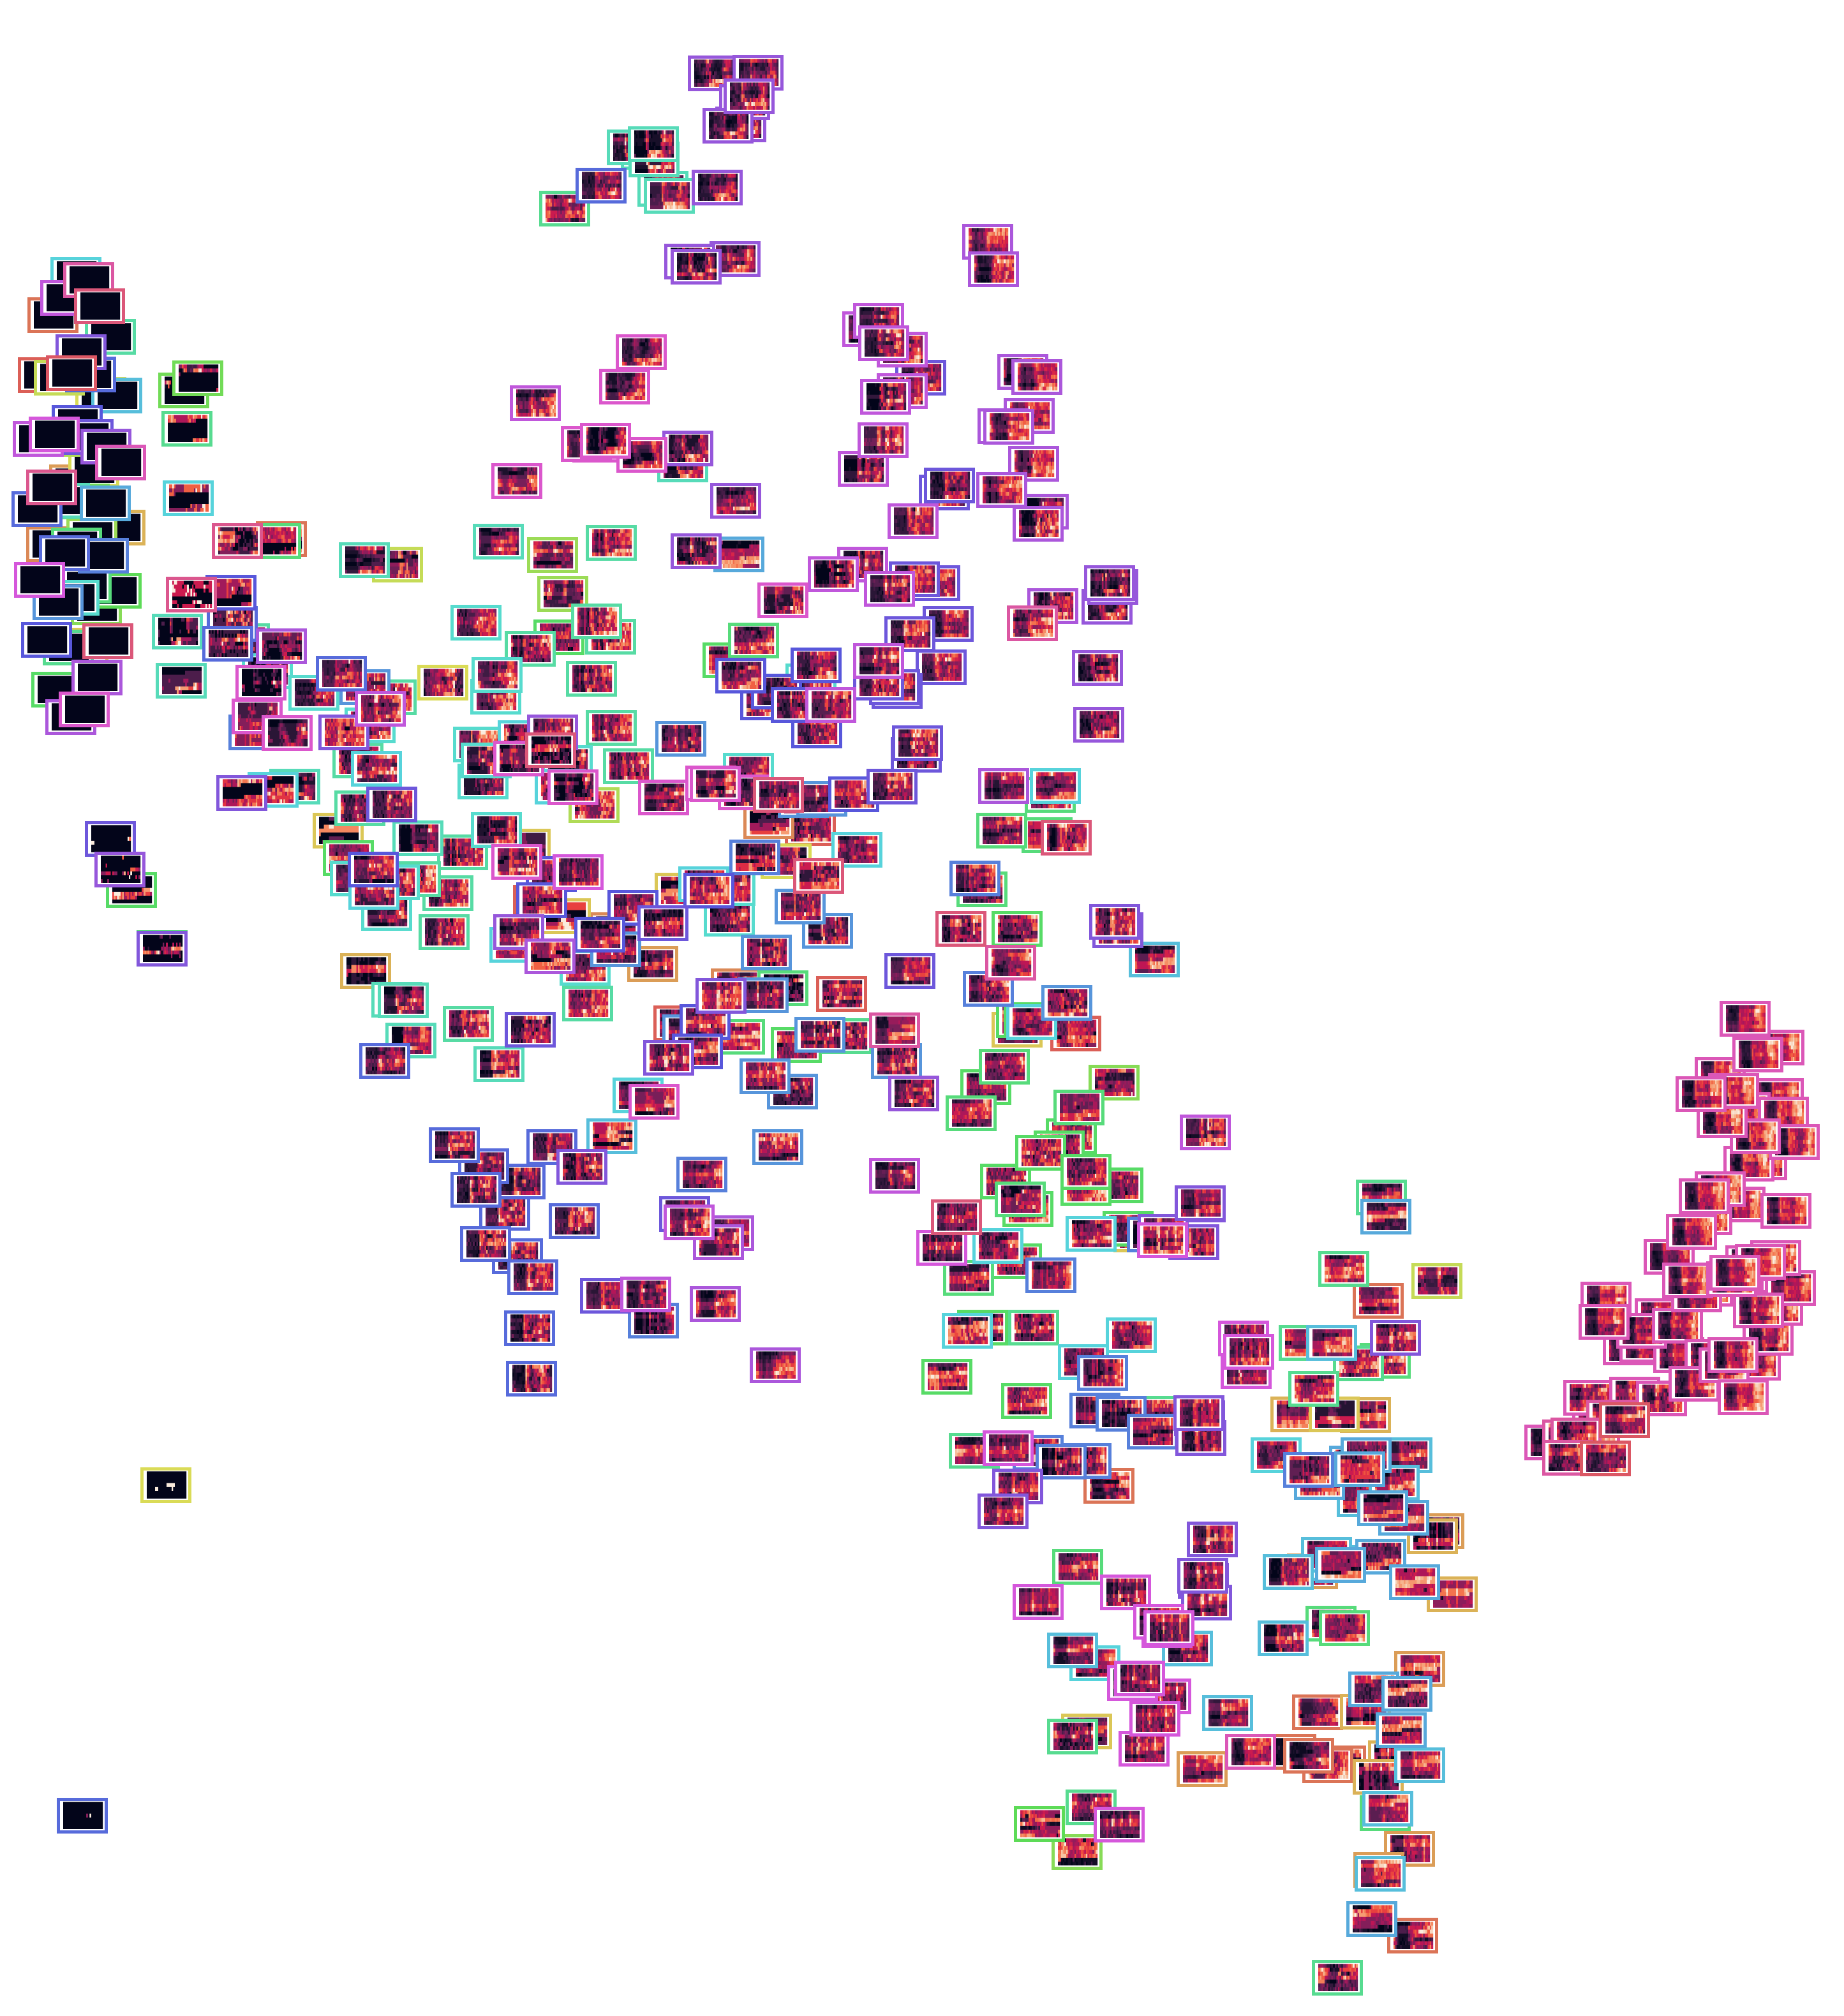
\includegraphics[width=.9\textwidth]{Figures/TSNE/TSNE_per_building/non_norm/img_scatter_allall.png}
	\label{fig:tsne_pb_img_scatter_allall}
\end{figure}

\subsubsection{Normalized load profiles}

To solve the issue mentioned in subsection \ref{ssec:res_pb_lp} have to normalize the data between 0 and 1.
The figure \ref{fig:tsne_pb_scatter_all_all} shows how normalizing samples affect the algorithm.

When comparing figures \ref{fig:tsne_scatter_non_norm_all} and \ref{fig:tsne_pb_img_scatter_allall},
it is possible to see that the samples on the latter are much closer to each other,
while it is still possible to see the individual clusters.
This could imply that the normalized usage pattern of users is more similar to the activation pattern of users.
A normalized activation pattern tells us at what part of the day the appliances will most likely be used,
and the activation pattern tells us how much will the appliance be used in each part of the day.
Based on that, we can conclude the time when the appliance is used is more consistent than how much it will be used. 


\begin{figure}[H]
	\centering
	\caption{"Projection of normalised per-building load profiles"}
	\includegraphics[width=1.2\textwidth]{Figures/TSNE/TSNE_per_building/all/scatter_all_all.png}
	\label{fig:tsne_pb_scatter_all_all}
\end{figure}

The figure \ref{fig:tsne_pb_img_norm_scatter_allall} presents only the main cluster of samples.
Since the smaller cluster presents mostly low entropy data, it was cut out. 
If the reader wants to see the samples in the cluster, the very same cluster can be found on the far left in figure \ref{fig:tsne_pb_img_scatter_allall}.

\begin{figure}[H]
	\centering
	\caption{"Projection of normalised per-building load profiles with actual samples"}
	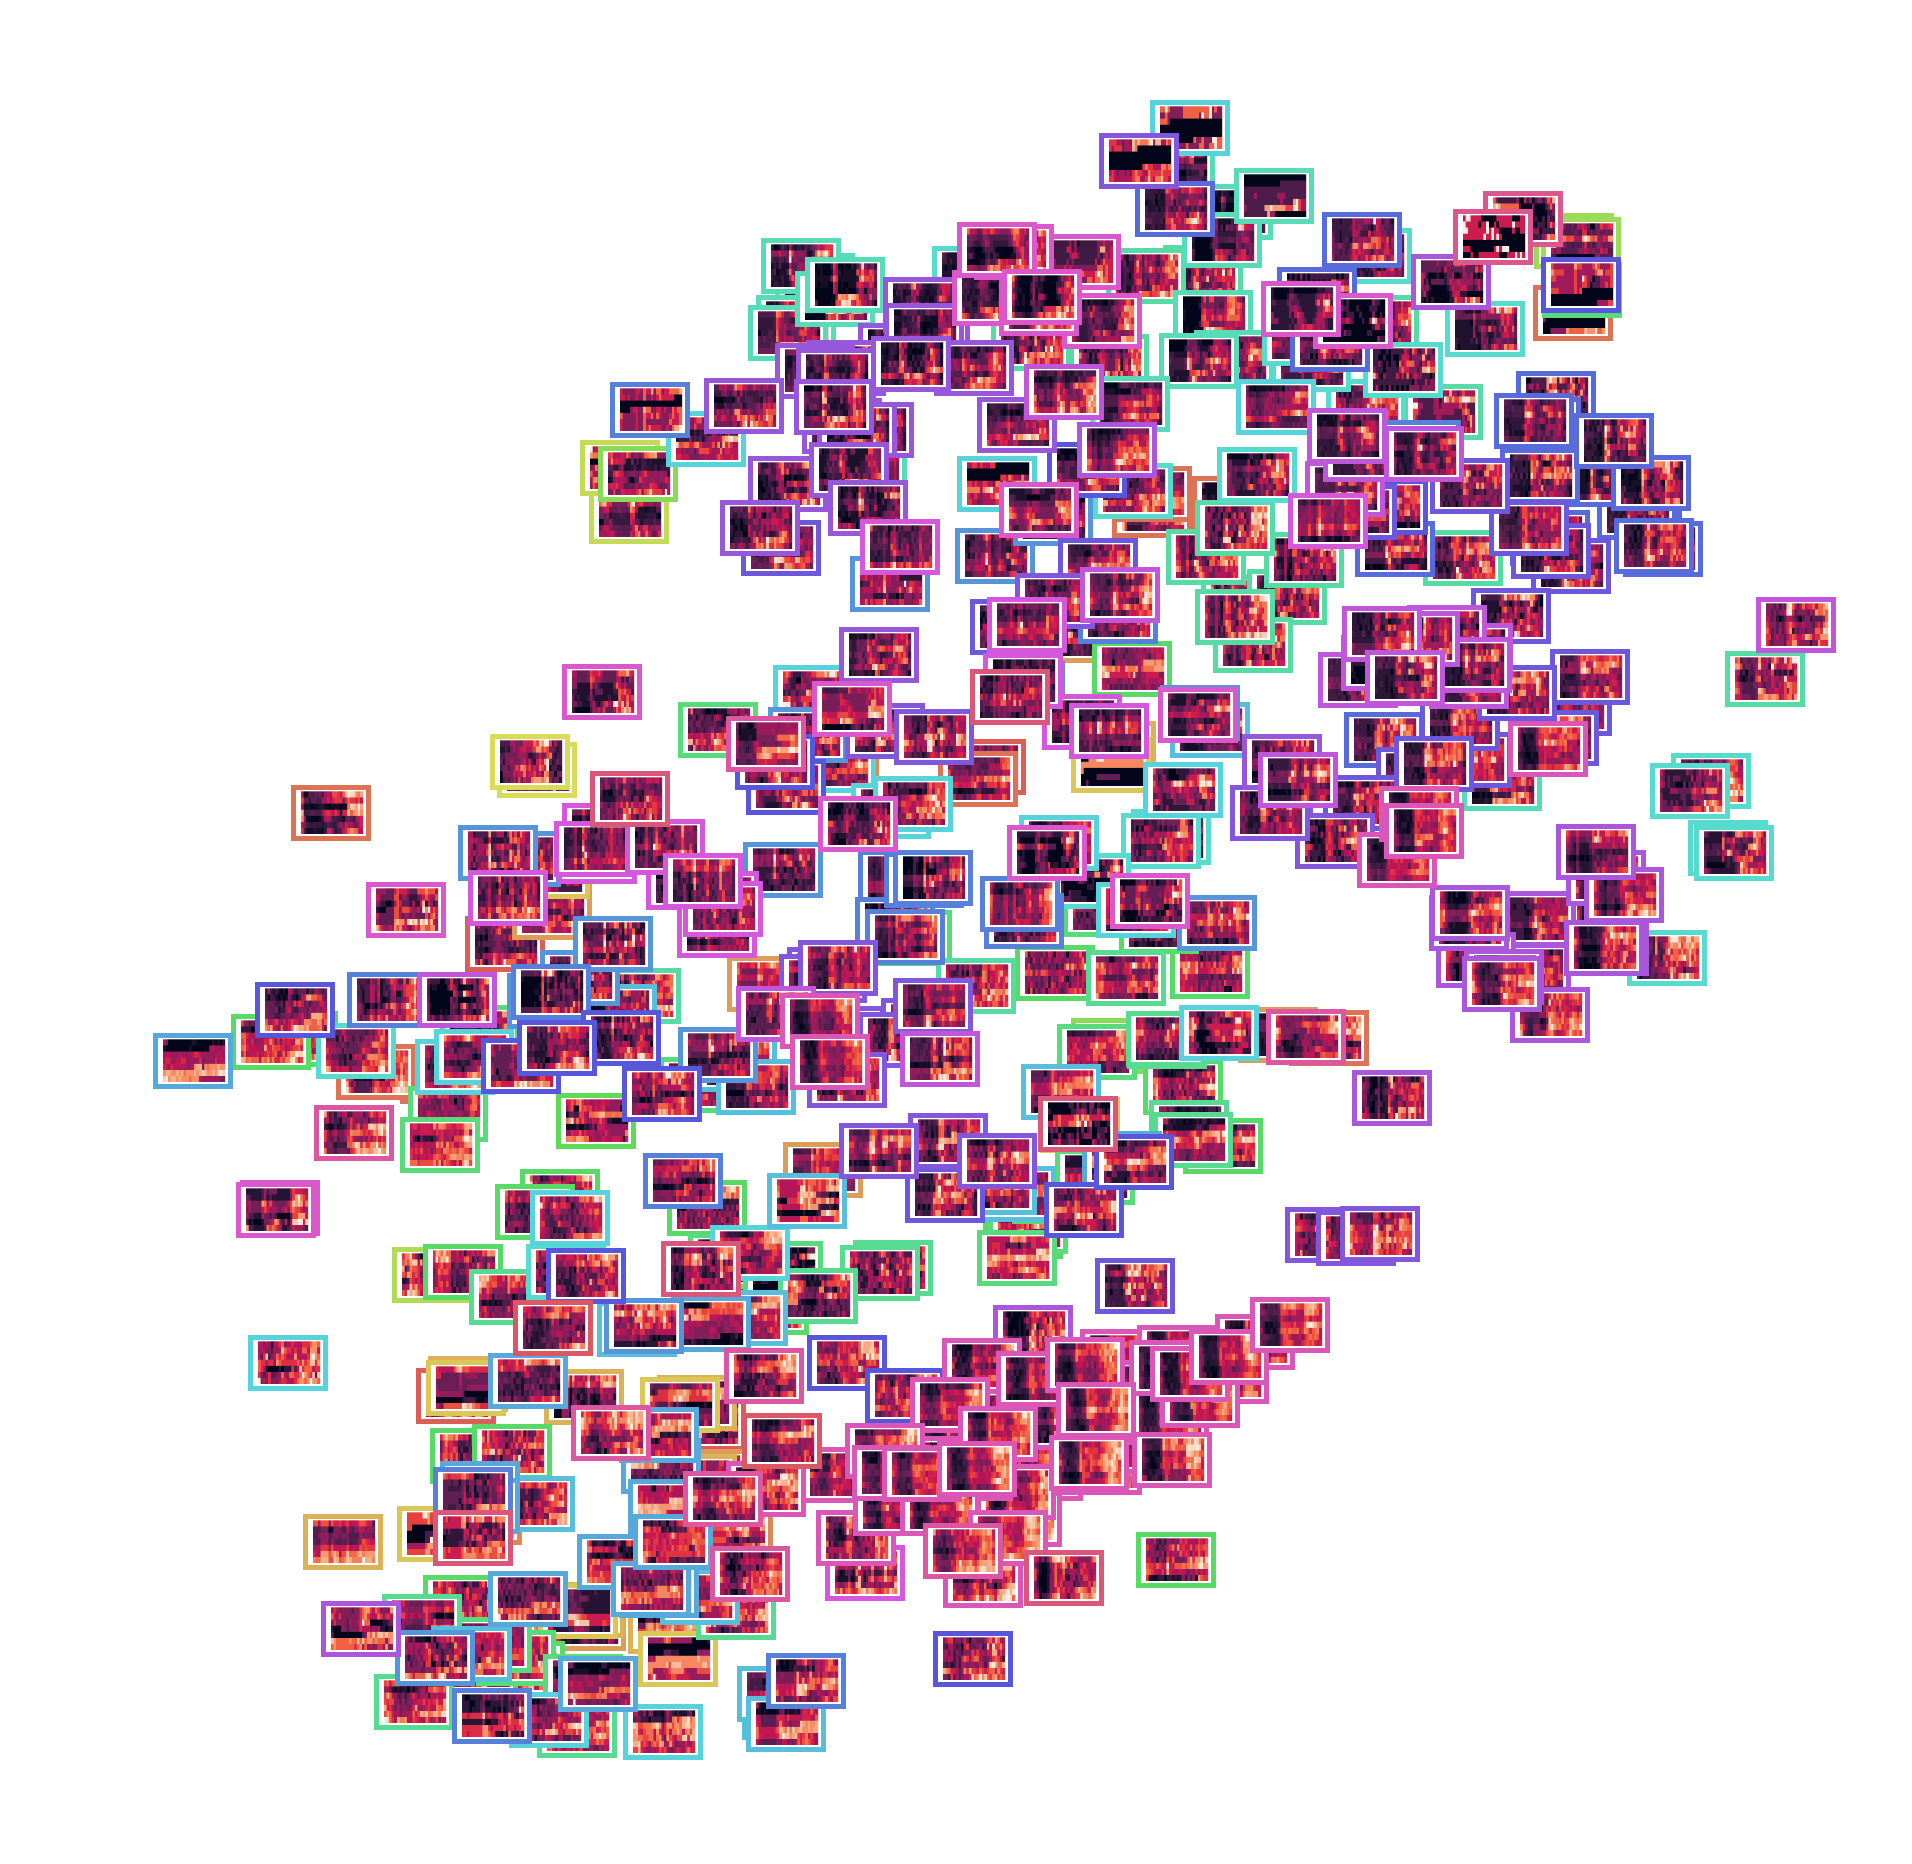
\includegraphics[width=.9\textwidth]{Figures/TSNE/TSNE_per_building/all/img_scatter_allall.png}
	\label{fig:tsne_pb_img_norm_scatter_allall}
\end{figure}

On figure \ref{fig:tsne_pb_img_norm_scatter_allall} it is possible to find various usage patterns. 
But the general pattern is that there is less activation during the night, then there is one peak during the morning and again once in the evening.
Some buildings are more active during the week and again others more during the weekend.
A lot of the data is from UK-DALE building 1 (pink box). 
It is possible to see that the building has one big cluster where activations are generally similar, then there are some outliers,
where the pattern completely changed. 
Albeit less obvious, the same happens overall buildings.
This happens due to events such as vacations, holidays or weather-induced behavioral changes.

\subsection{Per-appliance}

We can use per appliance load profiles to examine how different appliances 
are used in a single building, how a single appliance is being used across other buildings
or how many appliances are being used in many buildings.

Per appliance load profiles are built using sub-meter data,
meaning each load profile should present each appliance.

\subsubsection{Single appliance over many buildings}

Using one appliance and the building as a label,
allows us to examine how the same type of appliance is being used across different buildings.

Fridges are generally a bad indicator when it comes to user behavior since the user does not affect its operation. 
The only case when the user interacts with it is when opening the door and turning on the light inside. 
Usually, this event is dwarfed by the activations of a compressor. 
This also means that the usage pattern should be the same across all buildings. 
This can be seen on figure \ref{fig:tsne_pa_scatter_all_fridge}, 
where apart from REFIT building 1 and 11, there are no clusters.


\begin{figure}[H]
	\centering
	\caption{"Projection of fridge load profiles for various buildings"}
	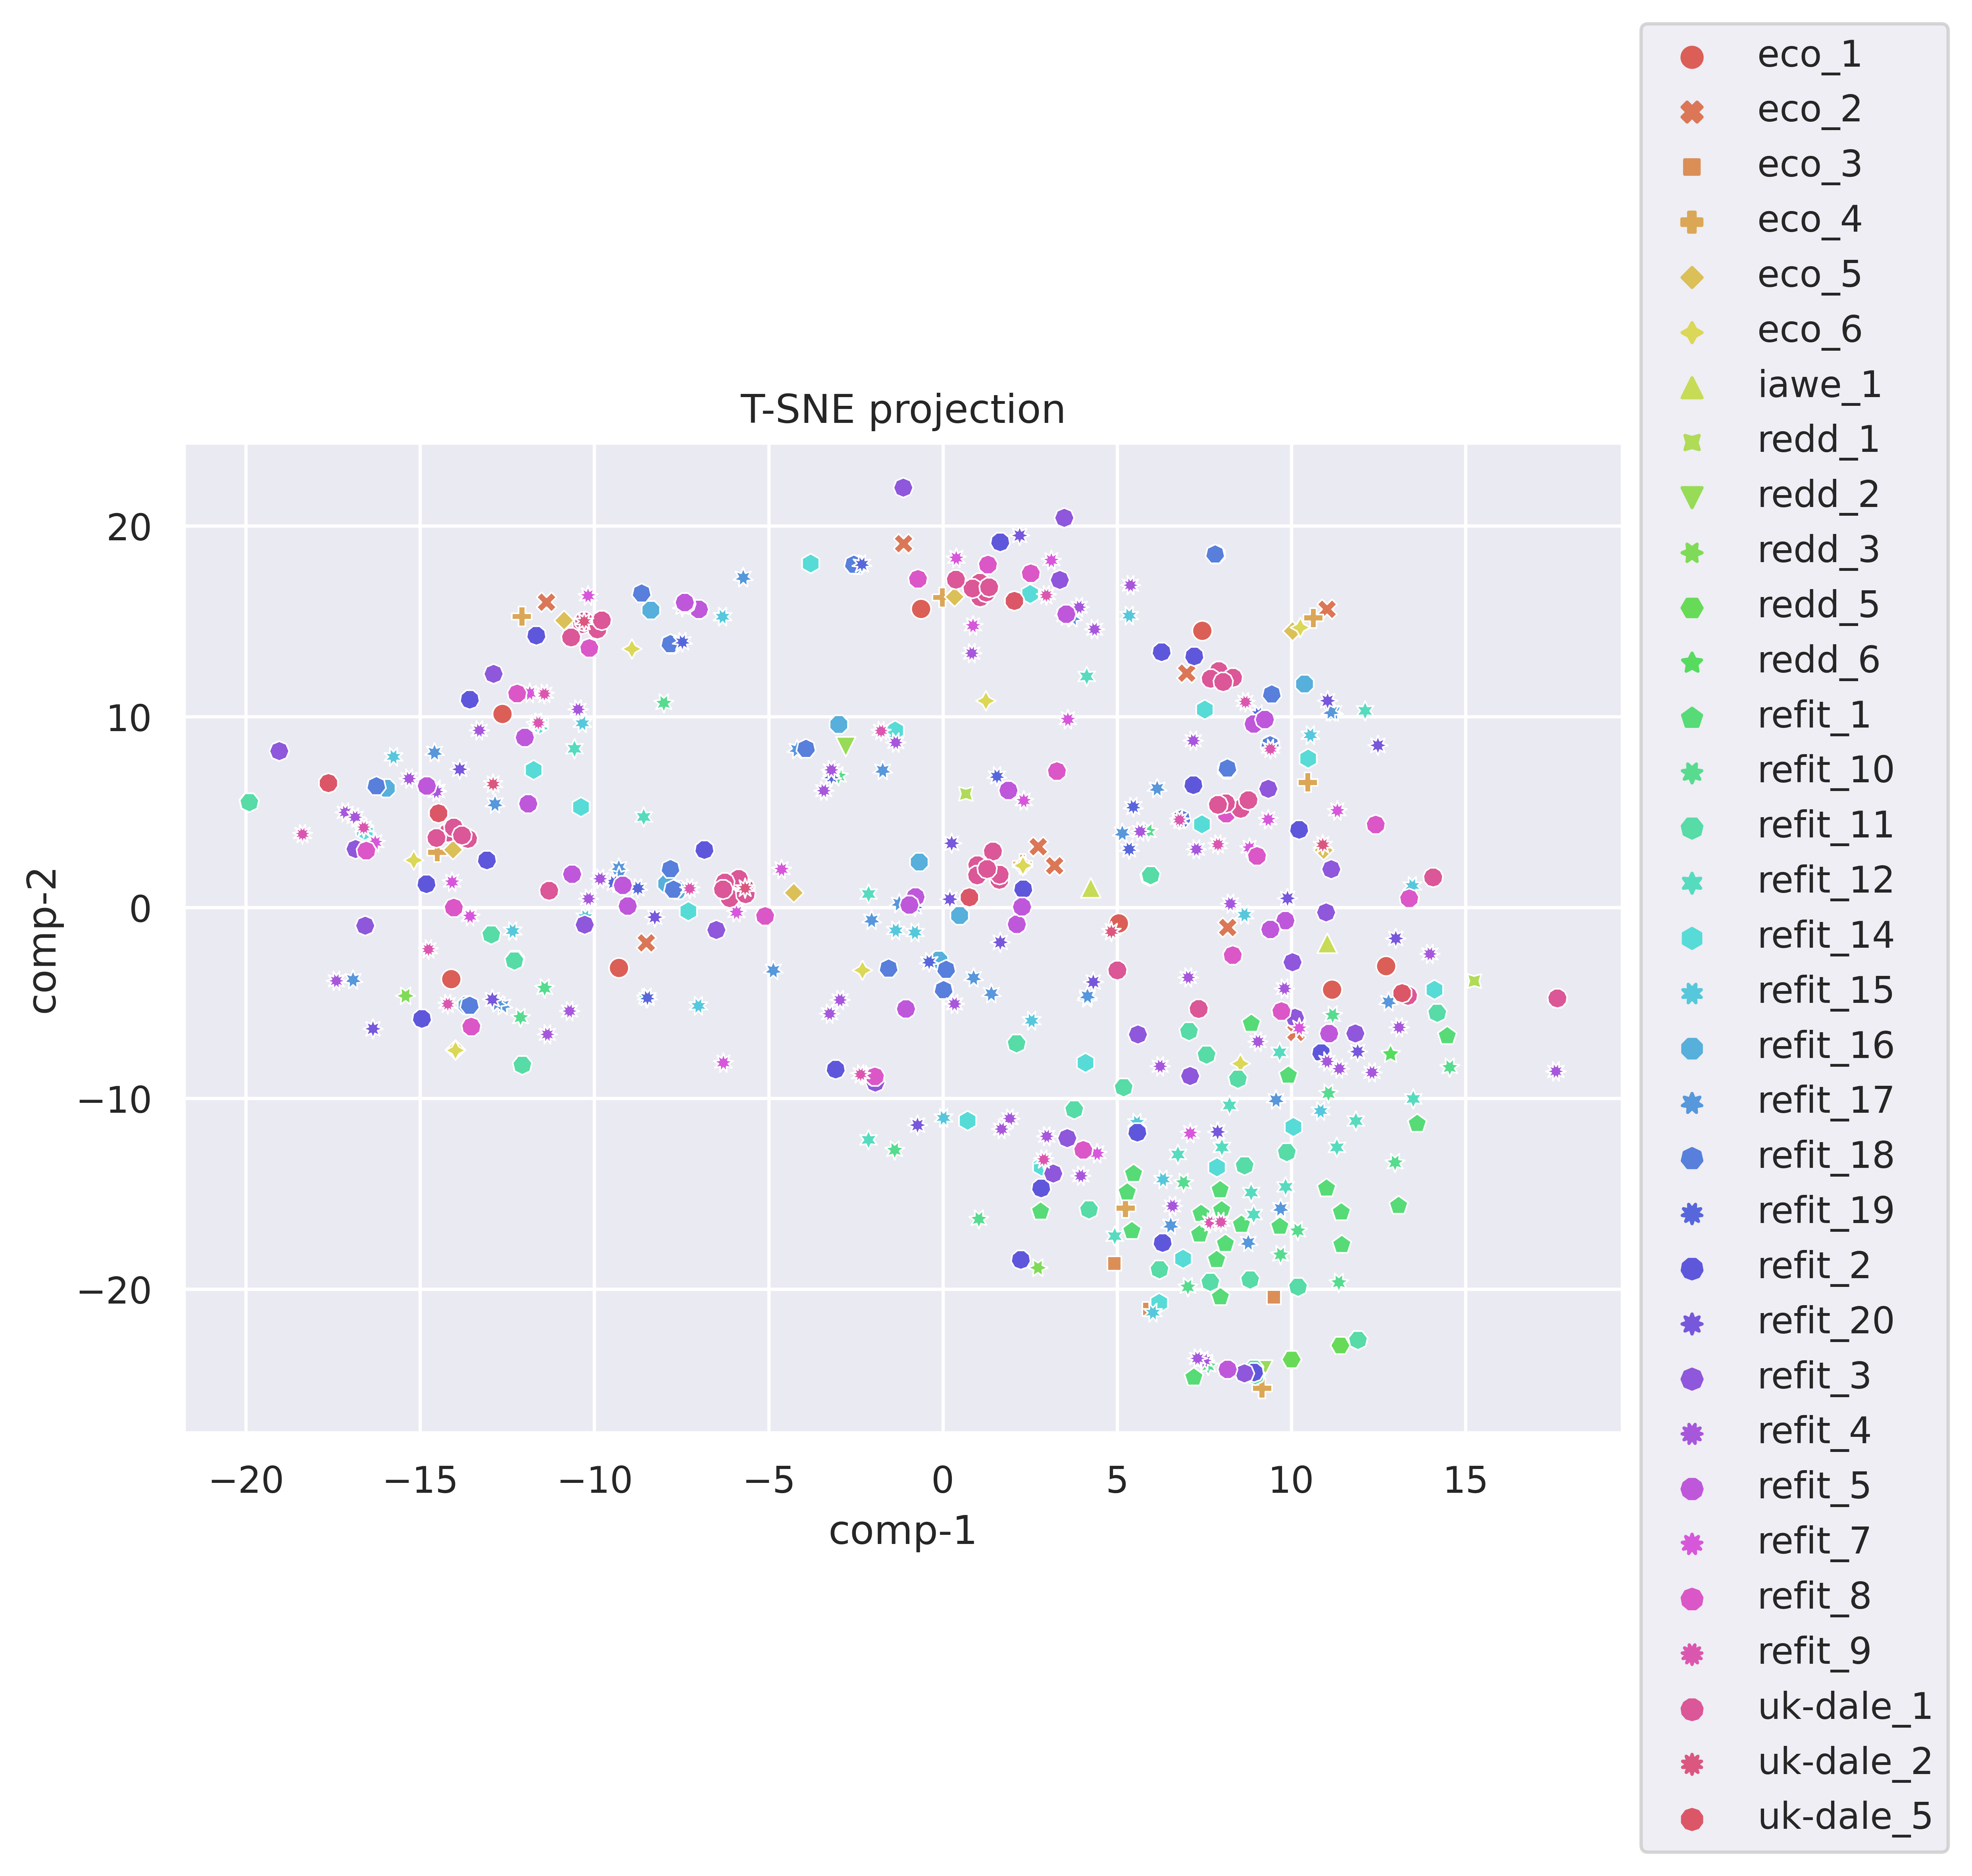
\includegraphics[width=1.2\textwidth]{Figures/TSNE/TSNE_per_appliance/all/scatter_all_fridge_freeezer_fridge freezer.png}
	\label{fig:tsne_pa_scatter_all_fridge}
\end{figure}

Figure \ref{fig:tsne_pa_img_scatter_all_fridge} Shows mostly bright images, apart from few outliers.
Load profiles scattered in a circle are generally less dynamic than the ones at the bottom.
The figure \ref{fig:tsne_pa_img_scatter_all_fridge} is a good example how even little to none human
interaction, load profiles can look a lot different. 
This could be due to different makes of the appliances, malfunctions of the appliance or the meter measuring it.

\begin{figure}[H]
	\centering
	\caption{"Projection of fridge load profiles for various buildings with actual samples"}
	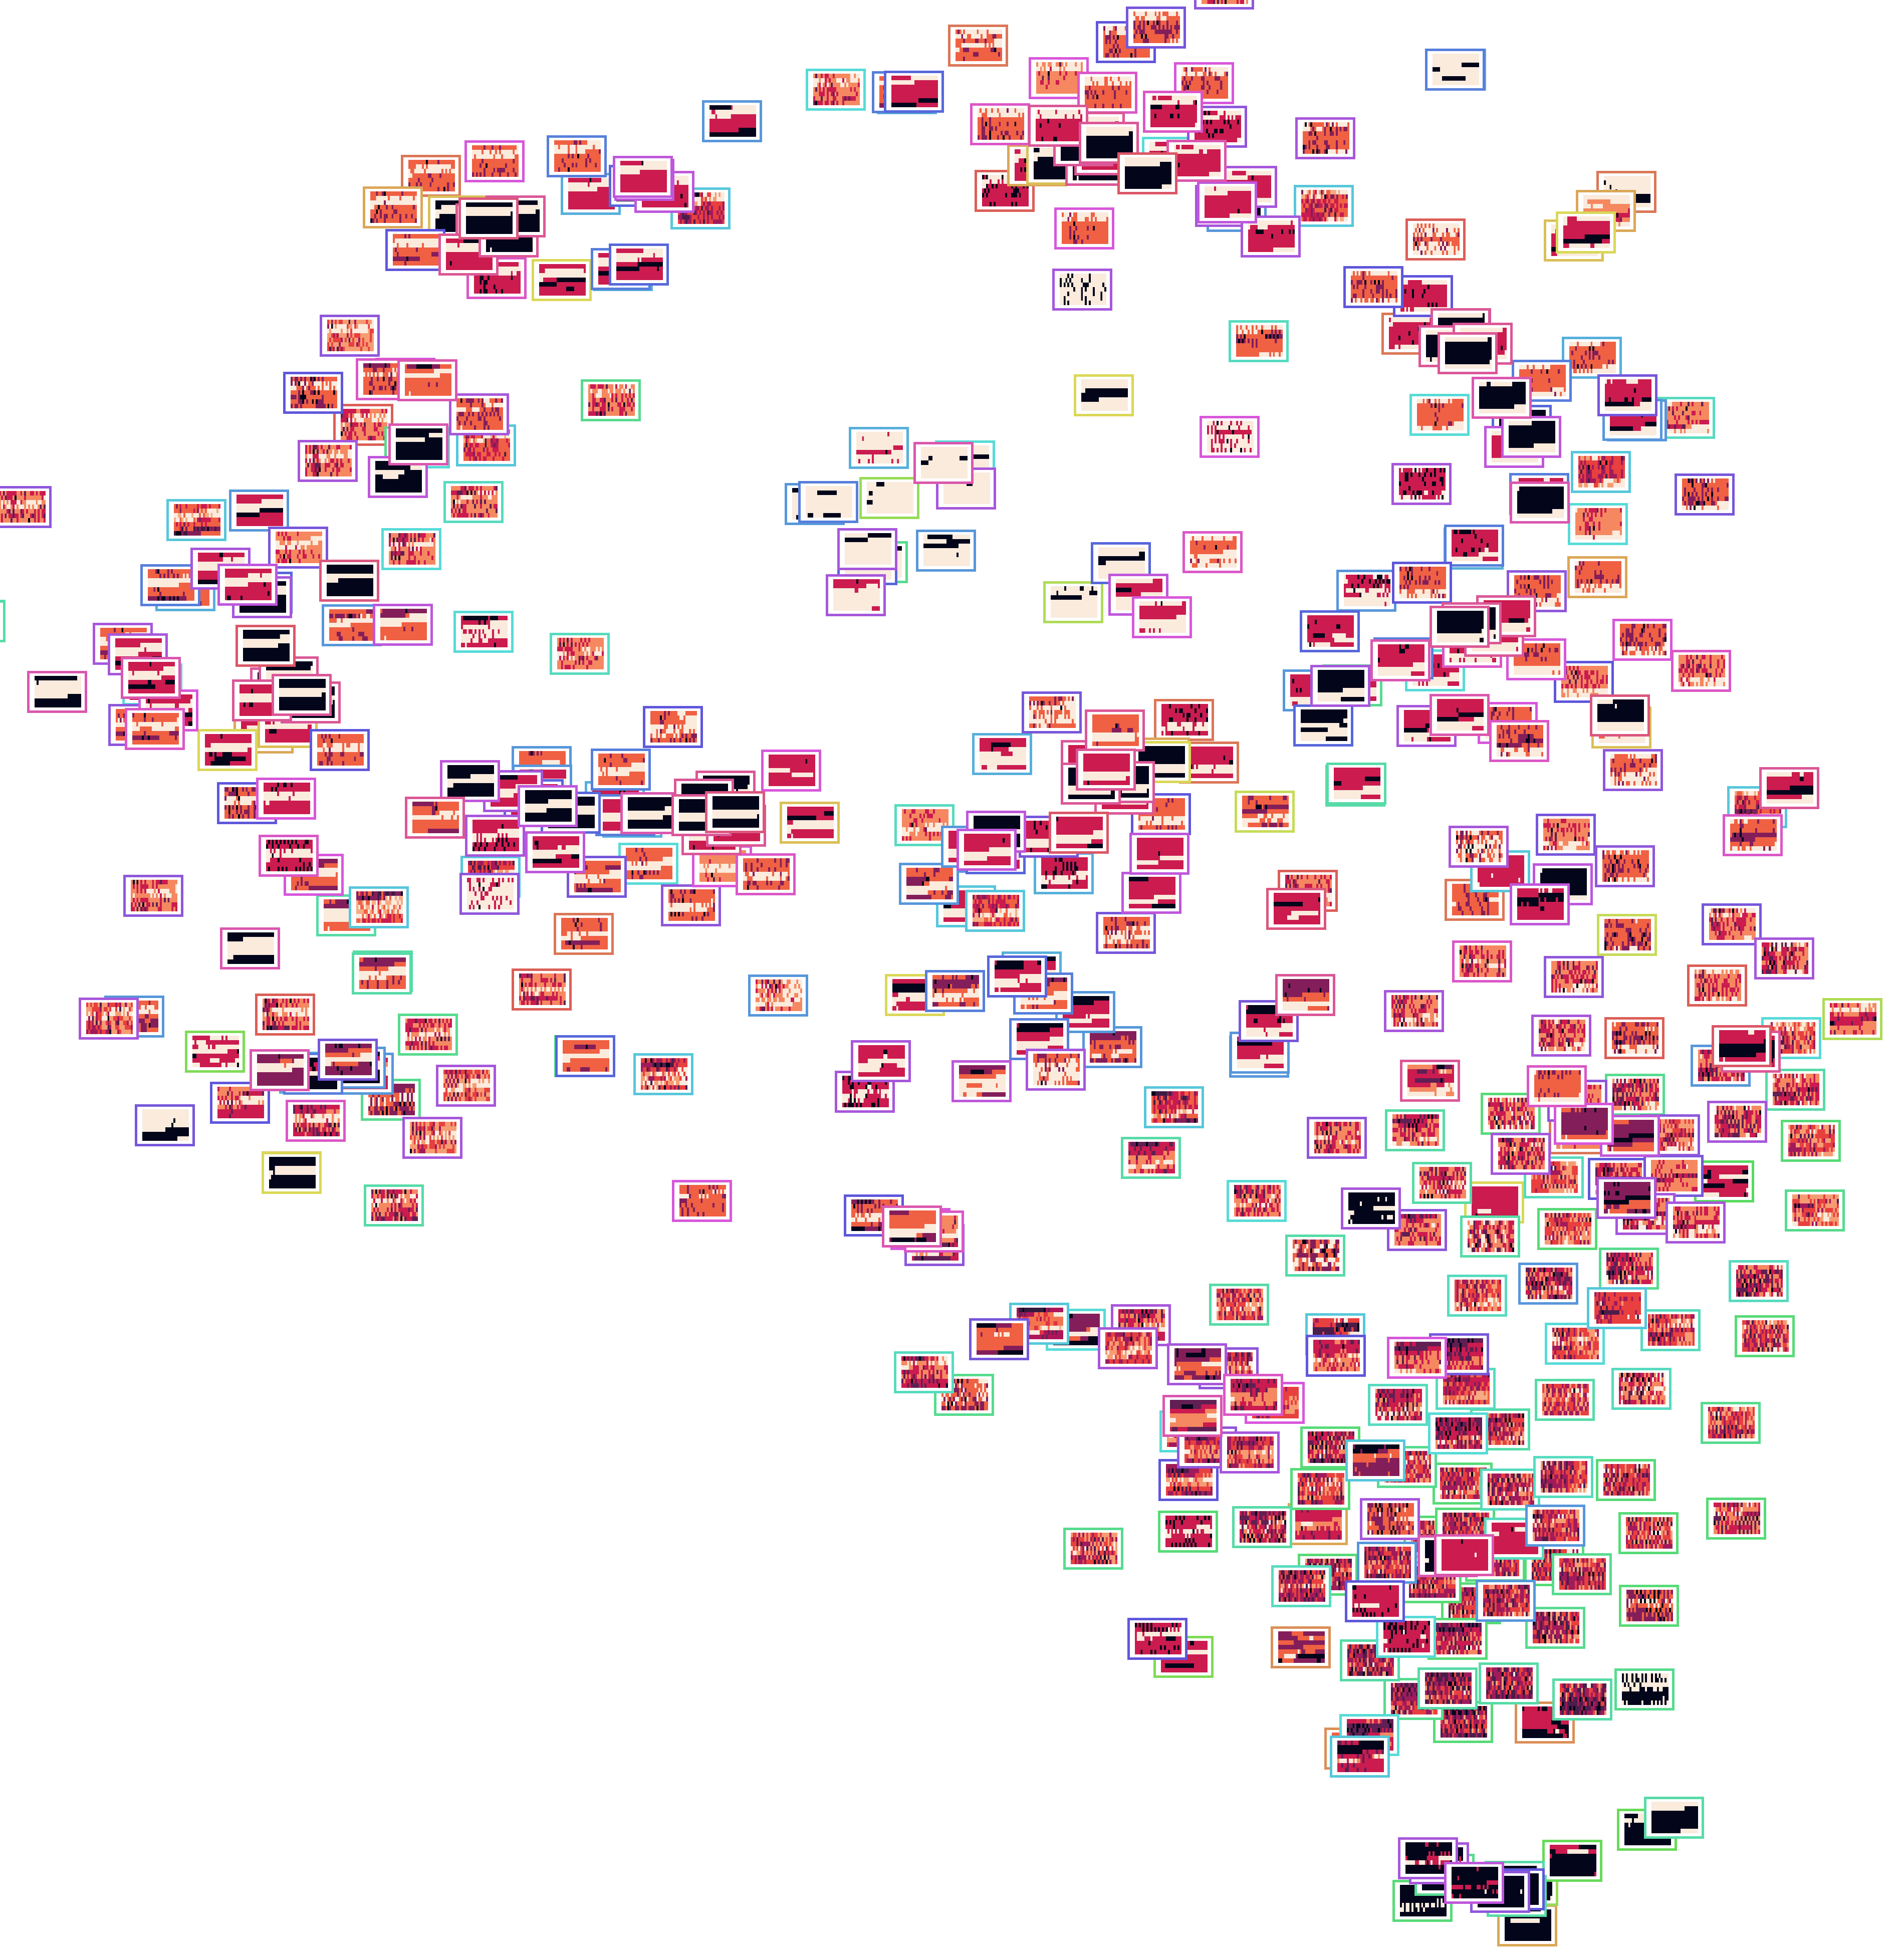
\includegraphics[width=.9\textwidth]{Figures/TSNE/TSNE_per_appliance/all/img_scatter_allfridge_freeezer_fridge freezer.png}
	\label{fig:tsne_pa_img_scatter_all_fridge}
\end{figure}

Figure \ref{fig:tsne_pa_scatter_all_kettle} shows how,
compared to fridges, kettles have much more clear clusters that are spaced out between each other. 
This could mean that every household uses a kettle a bit differently.
This cluster is a good example where we can see how strong is a routine of a user.
The closer together the clusters, the higher the routine since samples have to be 
close to each other.

\begin{figure}[H]
	\centering
	\caption{"Projection of kettle load profiles for various buildings"}
	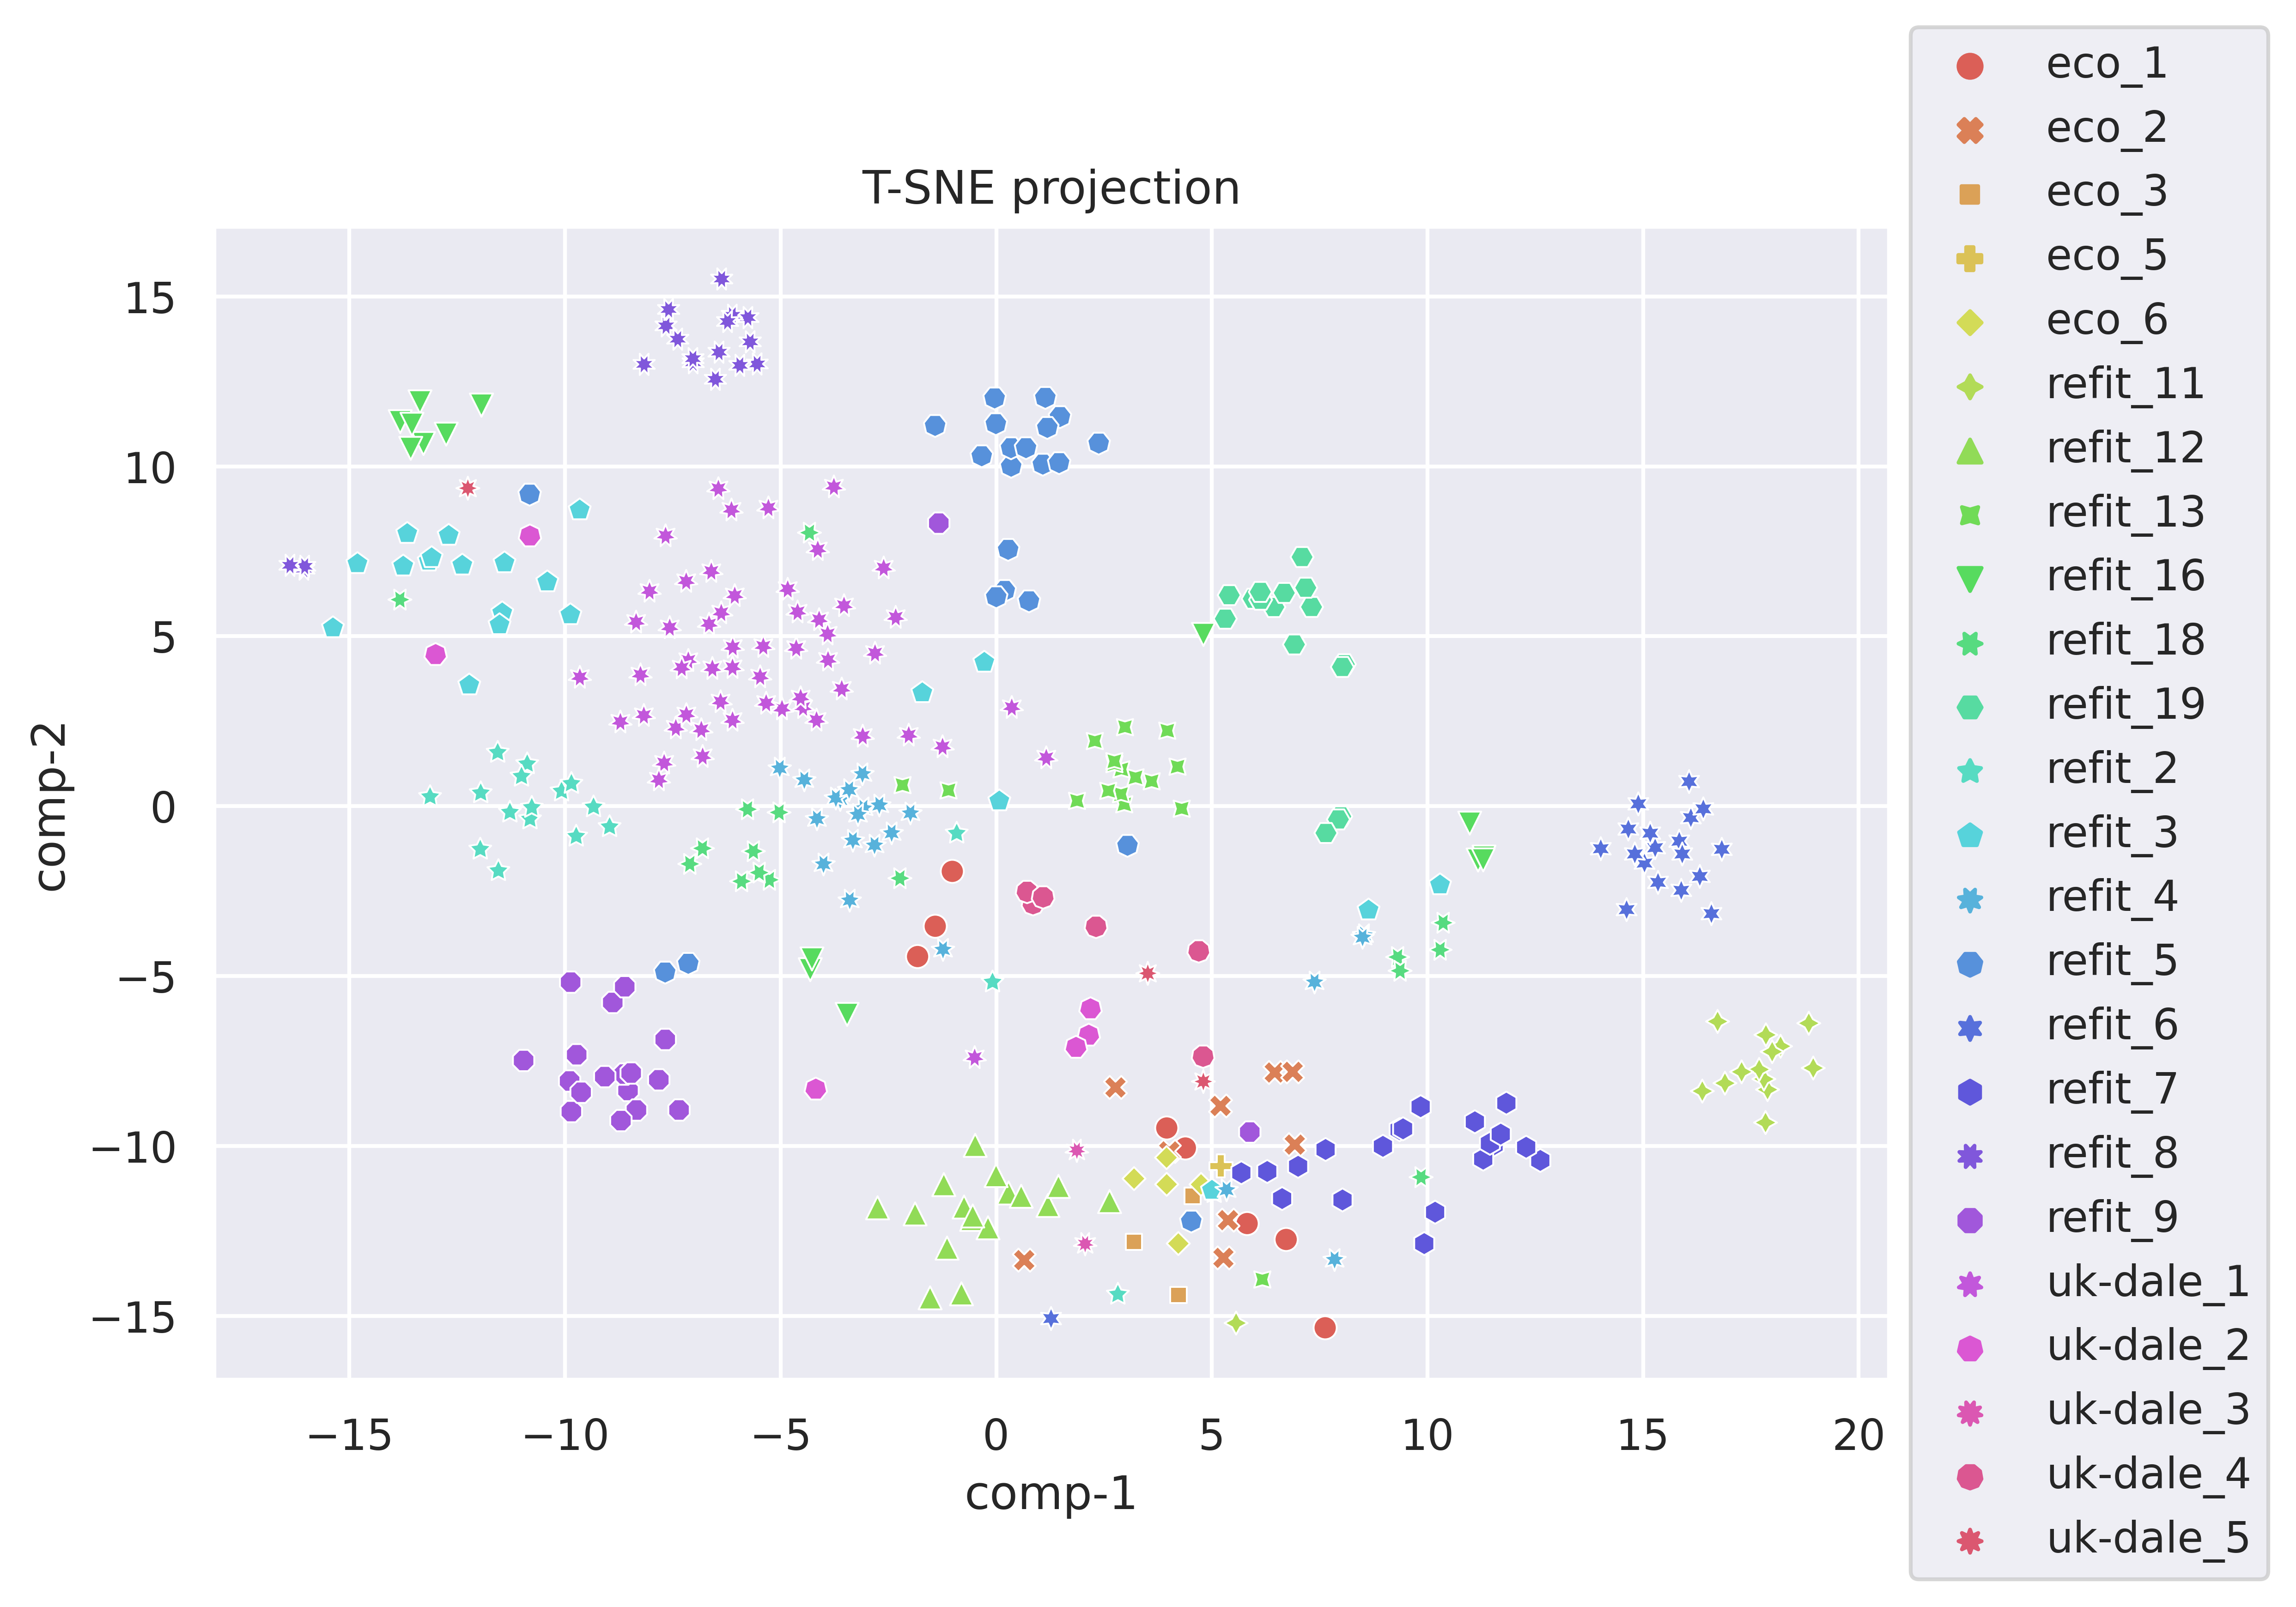
\includegraphics[width=1.2\textwidth]{Figures/TSNE/TSNE_per_appliance/all/scatter_all_kettle.png}
	\label{fig:tsne_pa_scatter_all_kettle}
\end{figure}

The figure \ref{fig:tsne_pa_img_scatter_all_kettle} shows us that images on the lower part 
of the plot contain less activity than the others. 
Load profiles that are closer together have more similar activation patterns.
Similar activations patterns are caused by similar behavior, which is essentially a routine.
This means that this projection could be used to calculate how much a behavior variate in time for each building.
This could be calculated by measuring the scattering of samples (variance) for each building.

If we find samples that always activate in the same morning buckets, we would see that they form a straight line on the y-axis.
This is the daily routine. One such example can be seen in figure \ref{fig:tsne_pa_scatter_all_kettle} in cluster refit 5 and refit 9, where we can see the lines and the pattern throughout the day. 
Since the routine is present the samples look more similar and are therefore closer together. 
This does not necessarily mean that closer the samples higher the routine.
They could also be together in case of the "ordered chaos" such as can be seen in the figure \ref{fig:tsne_pa_scatter_all_kettle} for building refit 16 and refit 8 where there is no pattern through the day.
So the scattering is not a precise metric when it comes to the routine, but it gives us a rough idea of its presence.
The strength of a routine is an important feature that will be used
in the next chapter to build an elderly care anomaly system.

\begin{figure}[H]
	\centering
	\caption{"Projection of kettle load profiles for various buildings with actual samples"}
	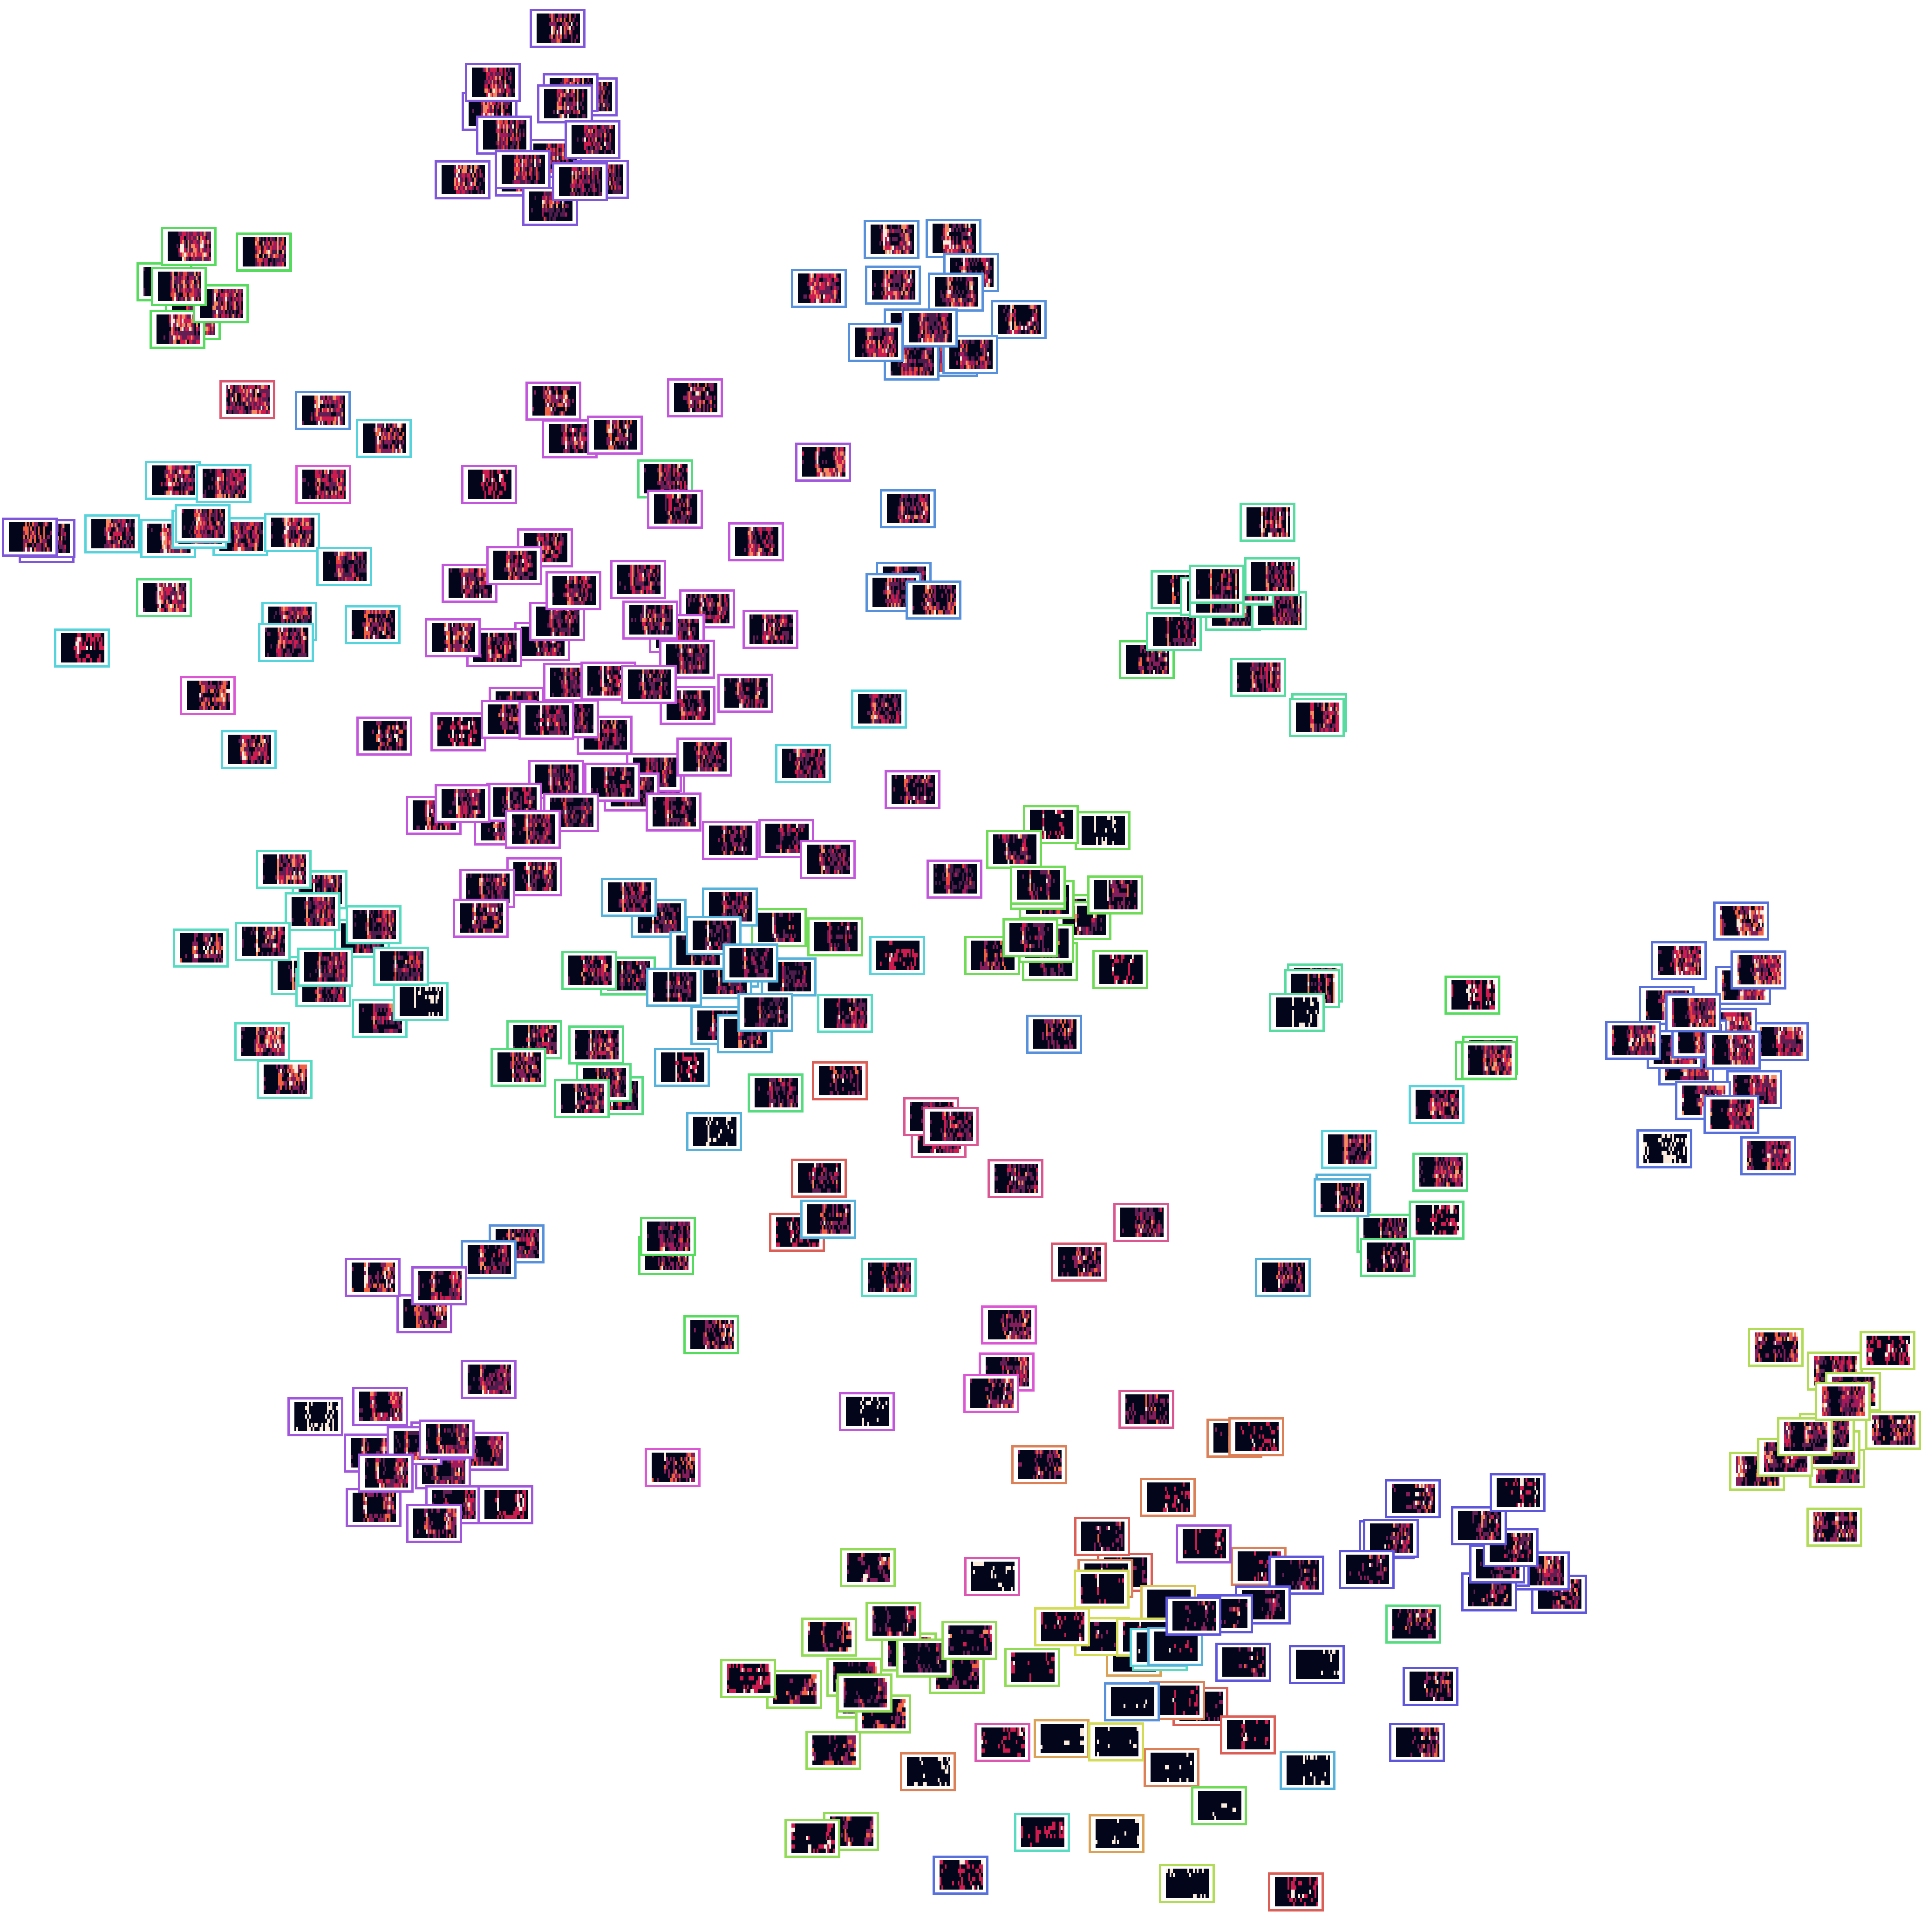
\includegraphics[width=.9\textwidth]{Figures/TSNE/TSNE_per_appliance/all/img_scatter_allkettle.png}
	\label{fig:tsne_pa_img_scatter_all_kettle}
\end{figure}

The figure \ref{fig:tsne_pa_scatter_all_microwave} shows that microwaves are again a bit different from the kettle.
They are more clustered than the fridges, and less than the kettles, even though they are used similarly.
This could be due to additional electronics such as a clock that are built into
the appliance. This could lead to some samples being registered as turned on due to 
a "dark" current. One other difference between the two is that microwave has more than one mode of operation.

\begin{figure}[H]
	\centering
	\caption{"Projection of microwave load profiles for various buildings"}
	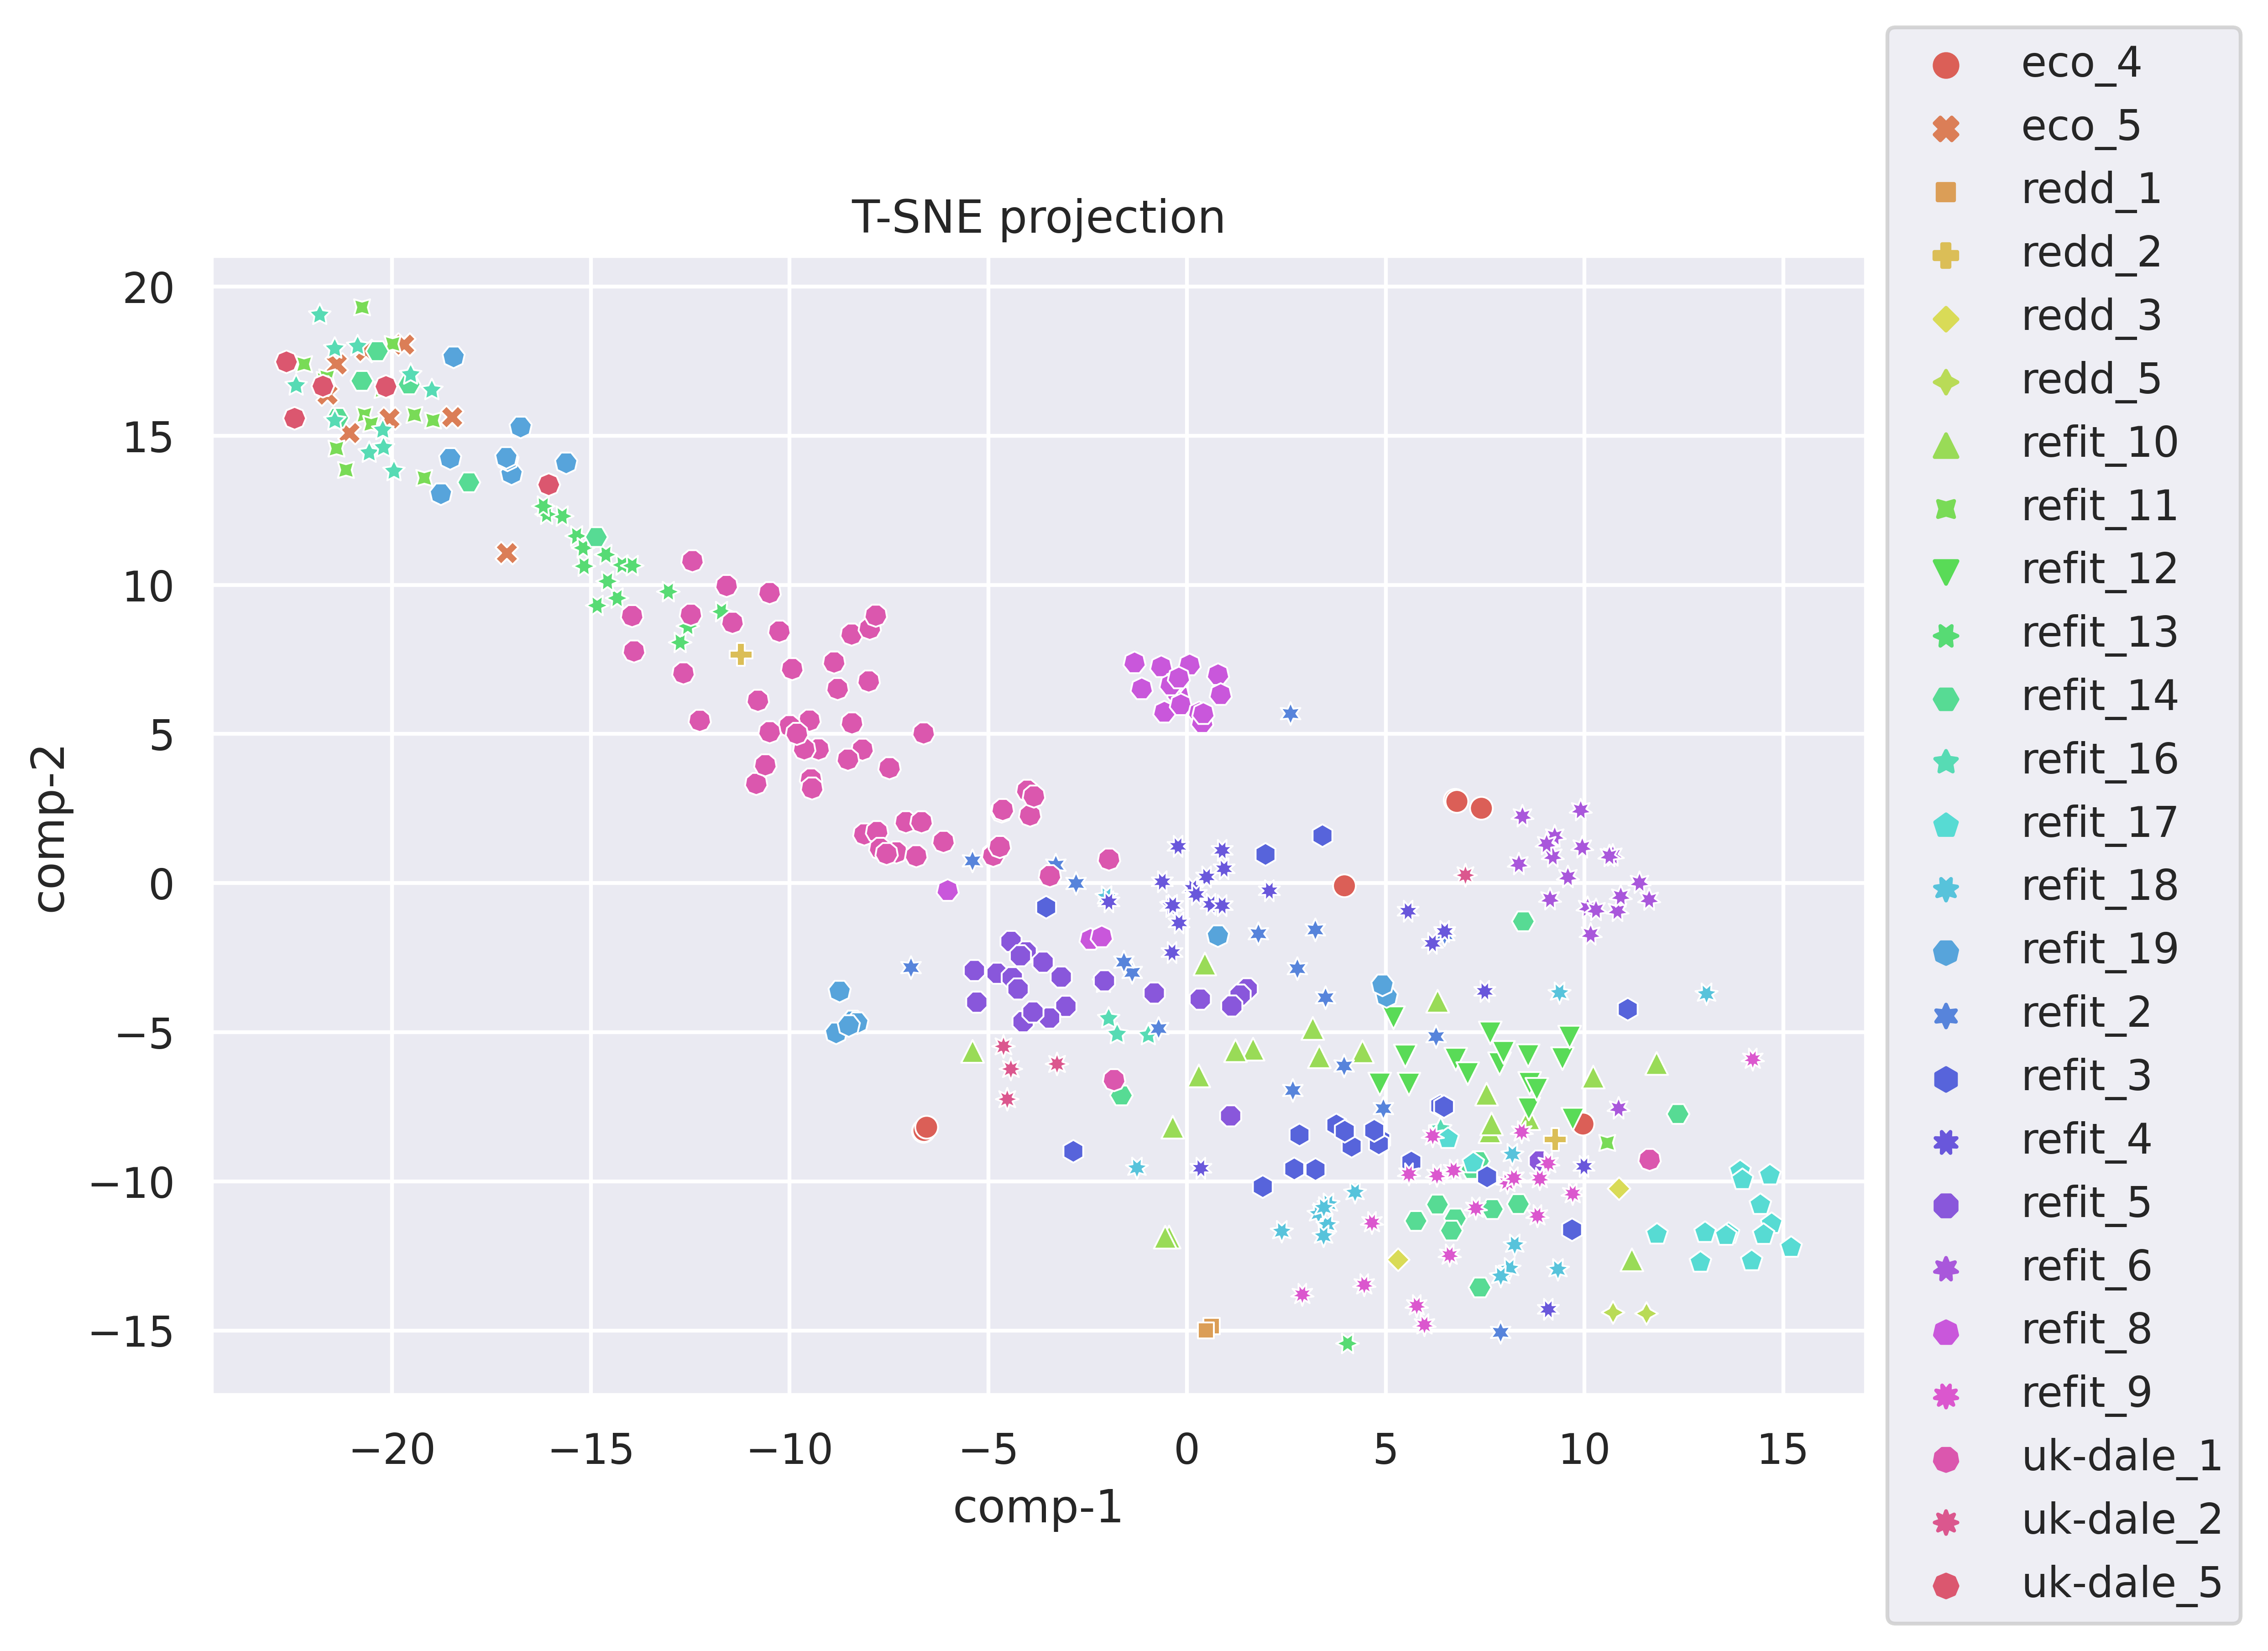
\includegraphics[width=1.2\textwidth]{Figures/TSNE/TSNE_per_appliance/all/scatter_all_microwave.png}
	\label{fig:tsne_pa_scatter_all_microwave}
\end{figure}

Figure \ref{fig:tsne_pa_img_scatter_all_microwave} shows the faulty samples could be the ones in the upper left part of the plot since they are too bright.
They do present a pattern, but it is questionable what it presents since it seems like it's turned on during the nighttime. 
Images at the other end show less lot less activity, which could indicate that
the household does not use microwaves as much. The most interesting load profiles are in the middle of the 
plot, where it is possible to observe clear activation patterns. 

\begin{figure}[H]
	\centering
	\caption{"Projection of microwave load profiles for various buildings with actual samples"}
	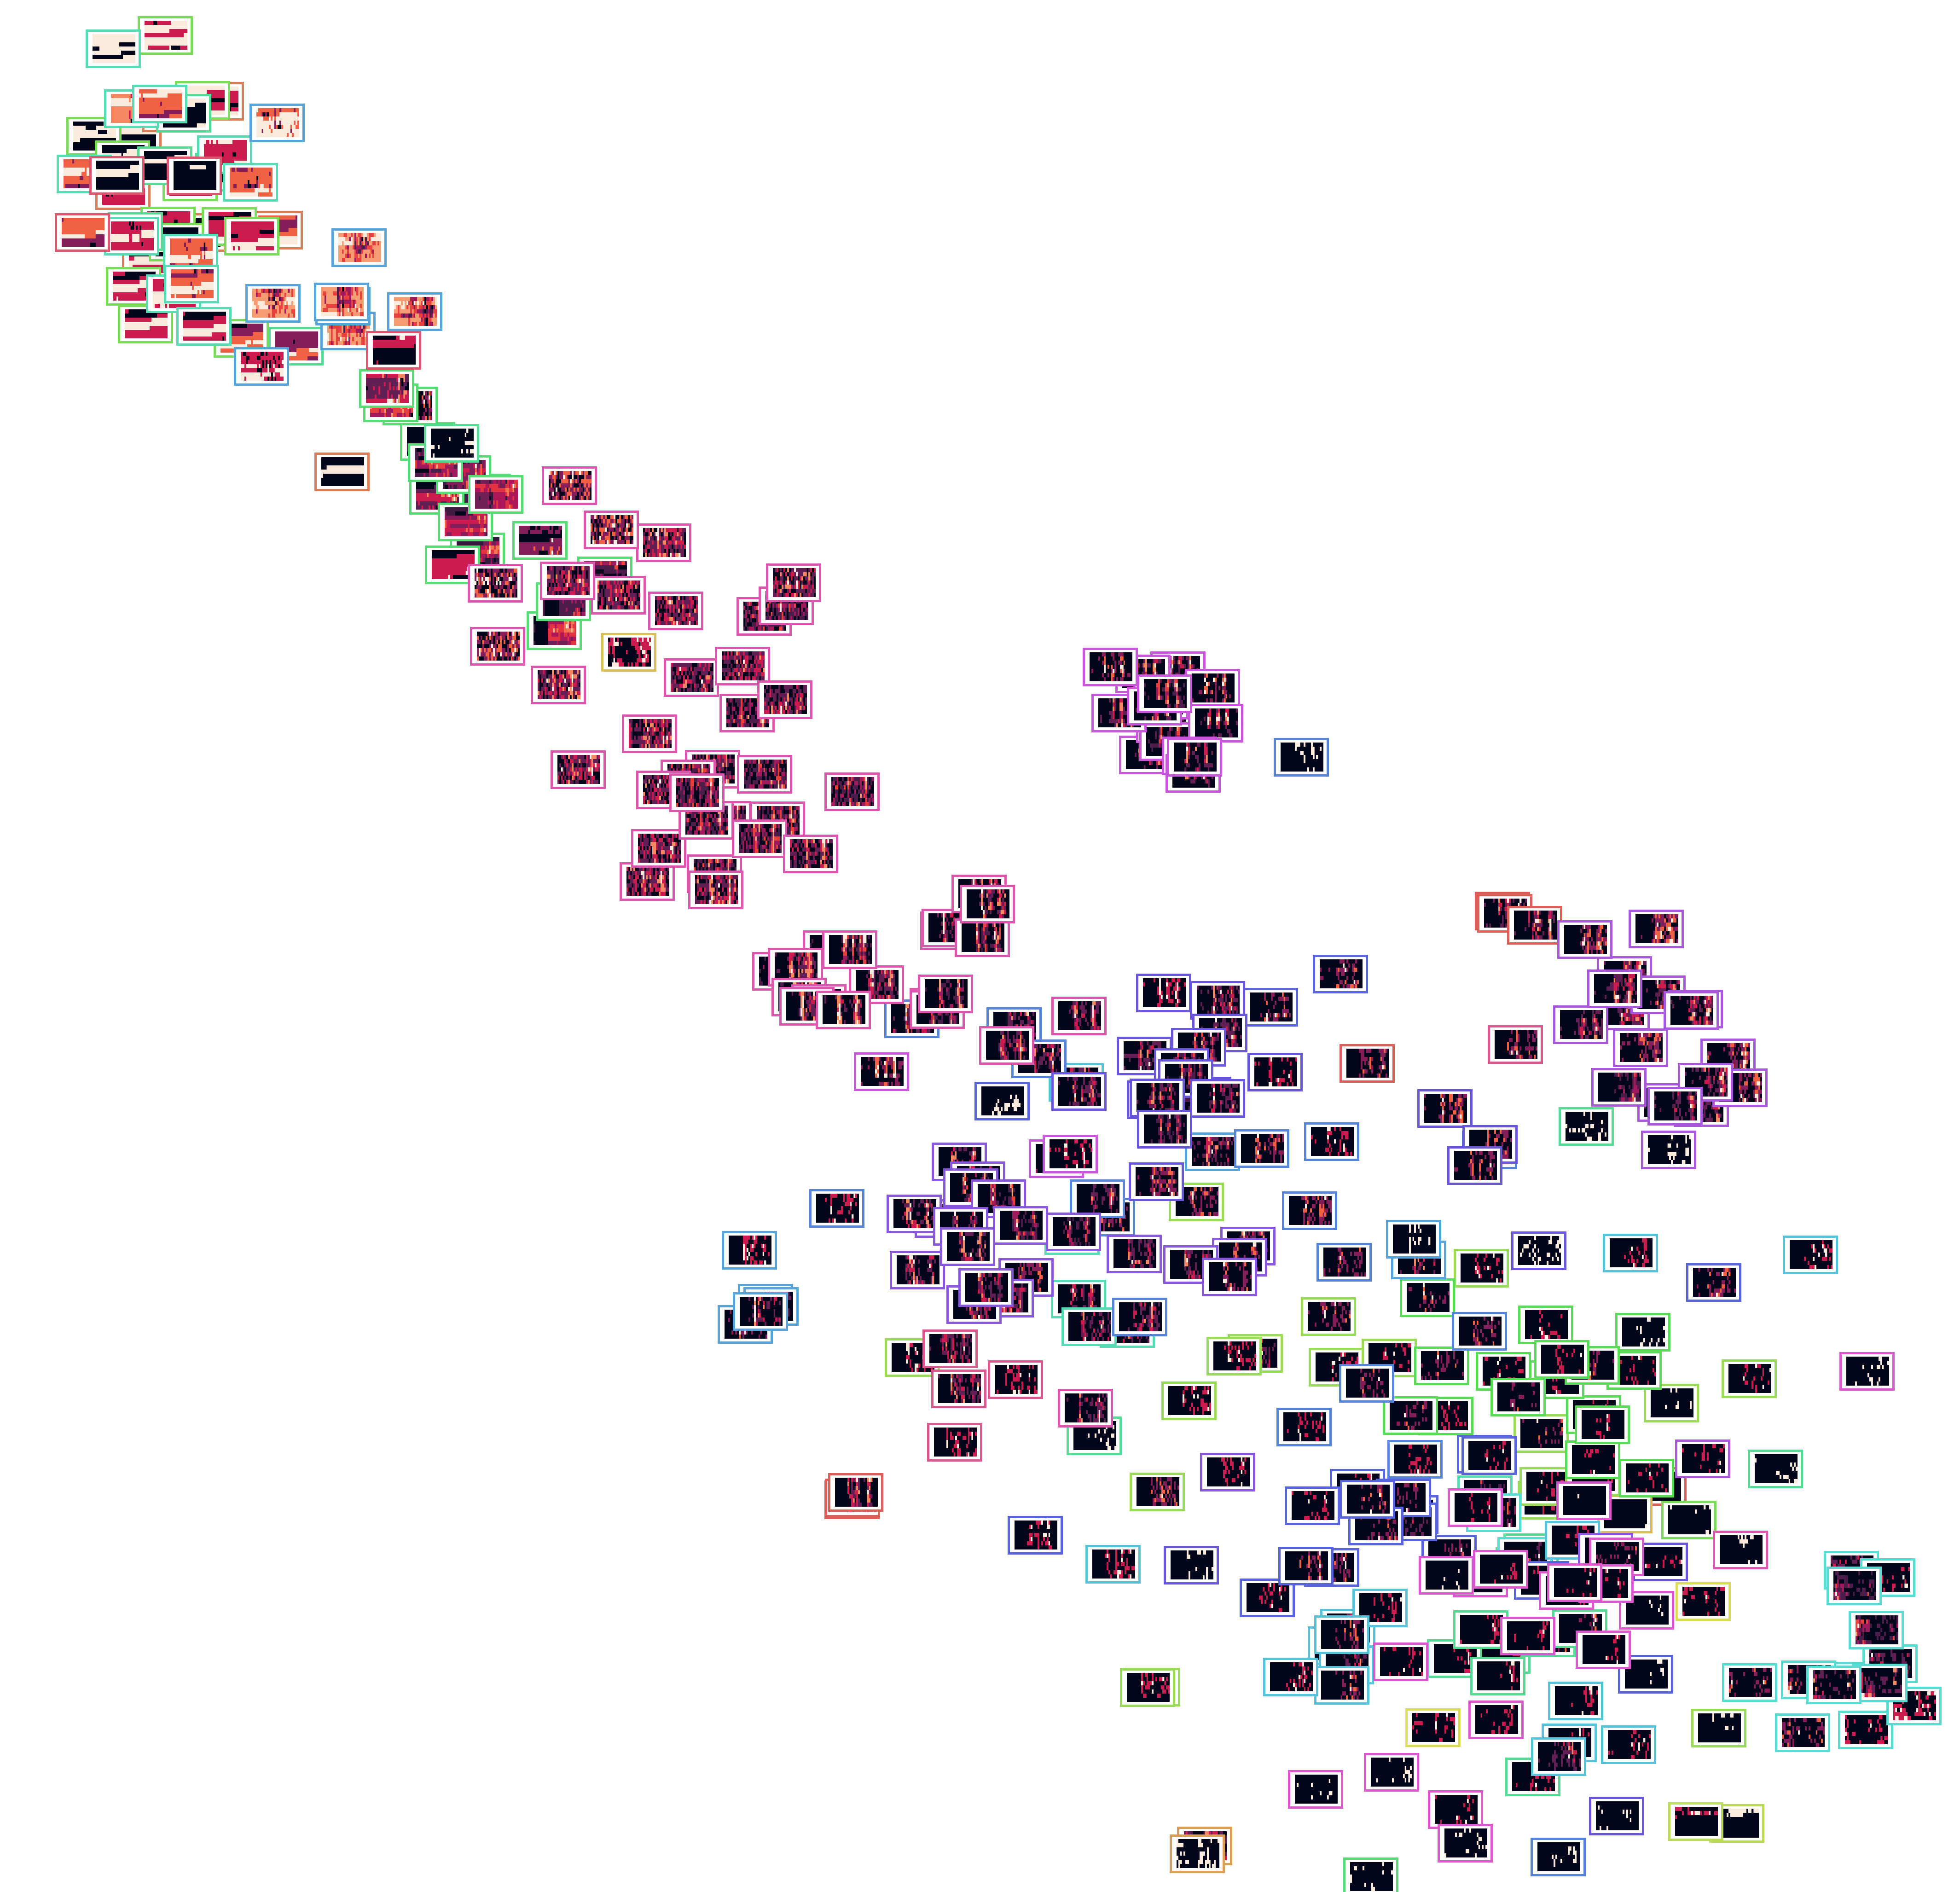
\includegraphics[width=.9\textwidth]{Figures/TSNE/TSNE_per_appliance/all/img_scatter_allmicrowave.png}
	\label{fig:tsne_pa_img_scatter_all_microwave}
\end{figure}

The last per-appliance example is television presented on figure \ref{fig:tsne_pa_scatter_all_tv}. 
Television was chosen since it is the most commonly occurring appliance.
Interestingly enough, televisions form nice clusters with a few outliers.
Clusters are separated but close together, this could mean that usage patterns are unique
but not that different from one another. 
The load profiles in some clusters are also close to each other, which could also indicate 
a higher routine.

\begin{figure}[H]
	\centering
	\caption{"Projection of TV load profiles for various buildings"}
	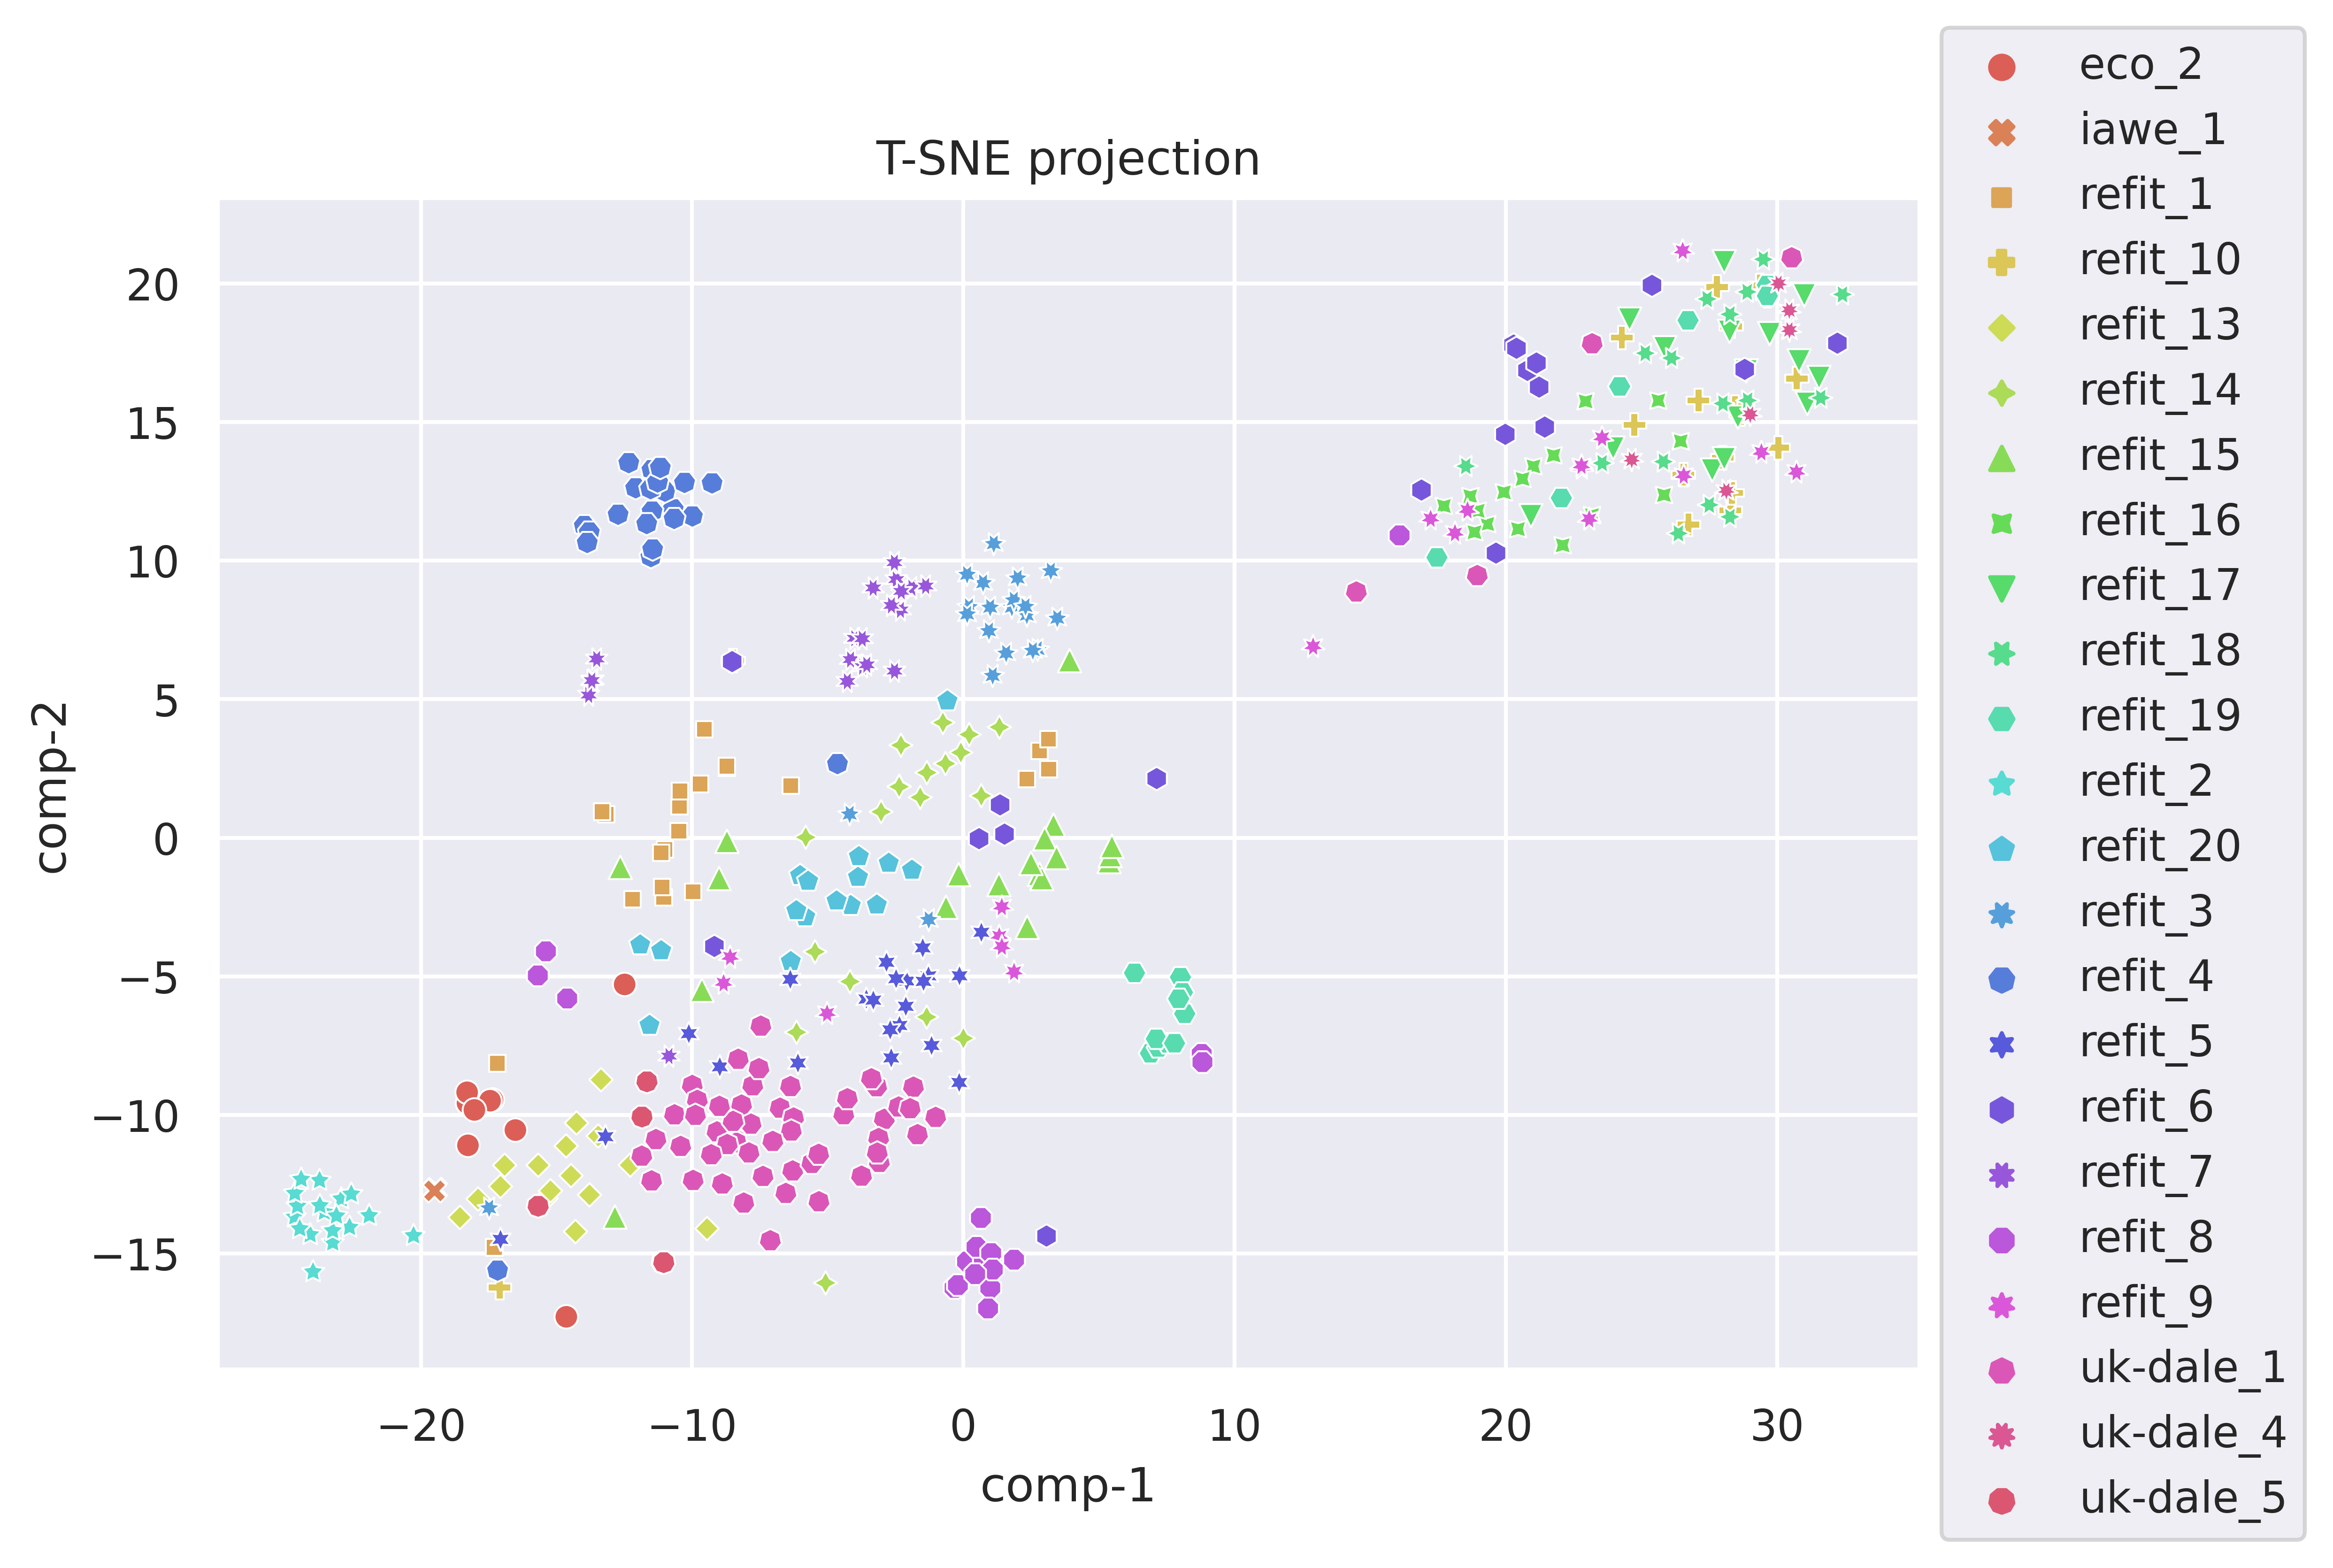
\includegraphics[width=1.2\textwidth]{Figures/TSNE/TSNE_per_appliance/all/scatter_all_television.png}
	\label{fig:tsne_pa_scatter_all_tv}
\end{figure}

The images on the figure \ref{fig:tsne_pa_img_scatter_all_tv} prove the fact that outliers' consumption is a lot different.
Again the bright images could be the results of faulty appliances, faulty meters or simply odd behavior.
The Figure \ref{fig:tsne_pa_img_scatter_all_tv} also enables us to see that TVs are primarily used 
in the evening hours. Outliers from the main cluster show slightly different behavior. One such 
example is the cyan blue cluster where appliances are mostly used in the morning hours. 
One other interesting observation can be made when looking at the purple cluster (the far low cluster).
Here TV is being consistently used in the early morning every day and this is portrayed as a straight line.
There could be two possible explanations for this.
First is simply a high routine of a user, who turns on the TV every morning to listen to the news or something similar.
The other is that TV updates itself every morning. This is probably not the case since updates do not occur on regular basis.
What is also interesting, is that the very same pattern can be observed on the sample from the other building (blue sample).

\begin{figure}[H]
	\centering
	\caption{"Projection of TV load profiles for various buildings with actual samples"}
	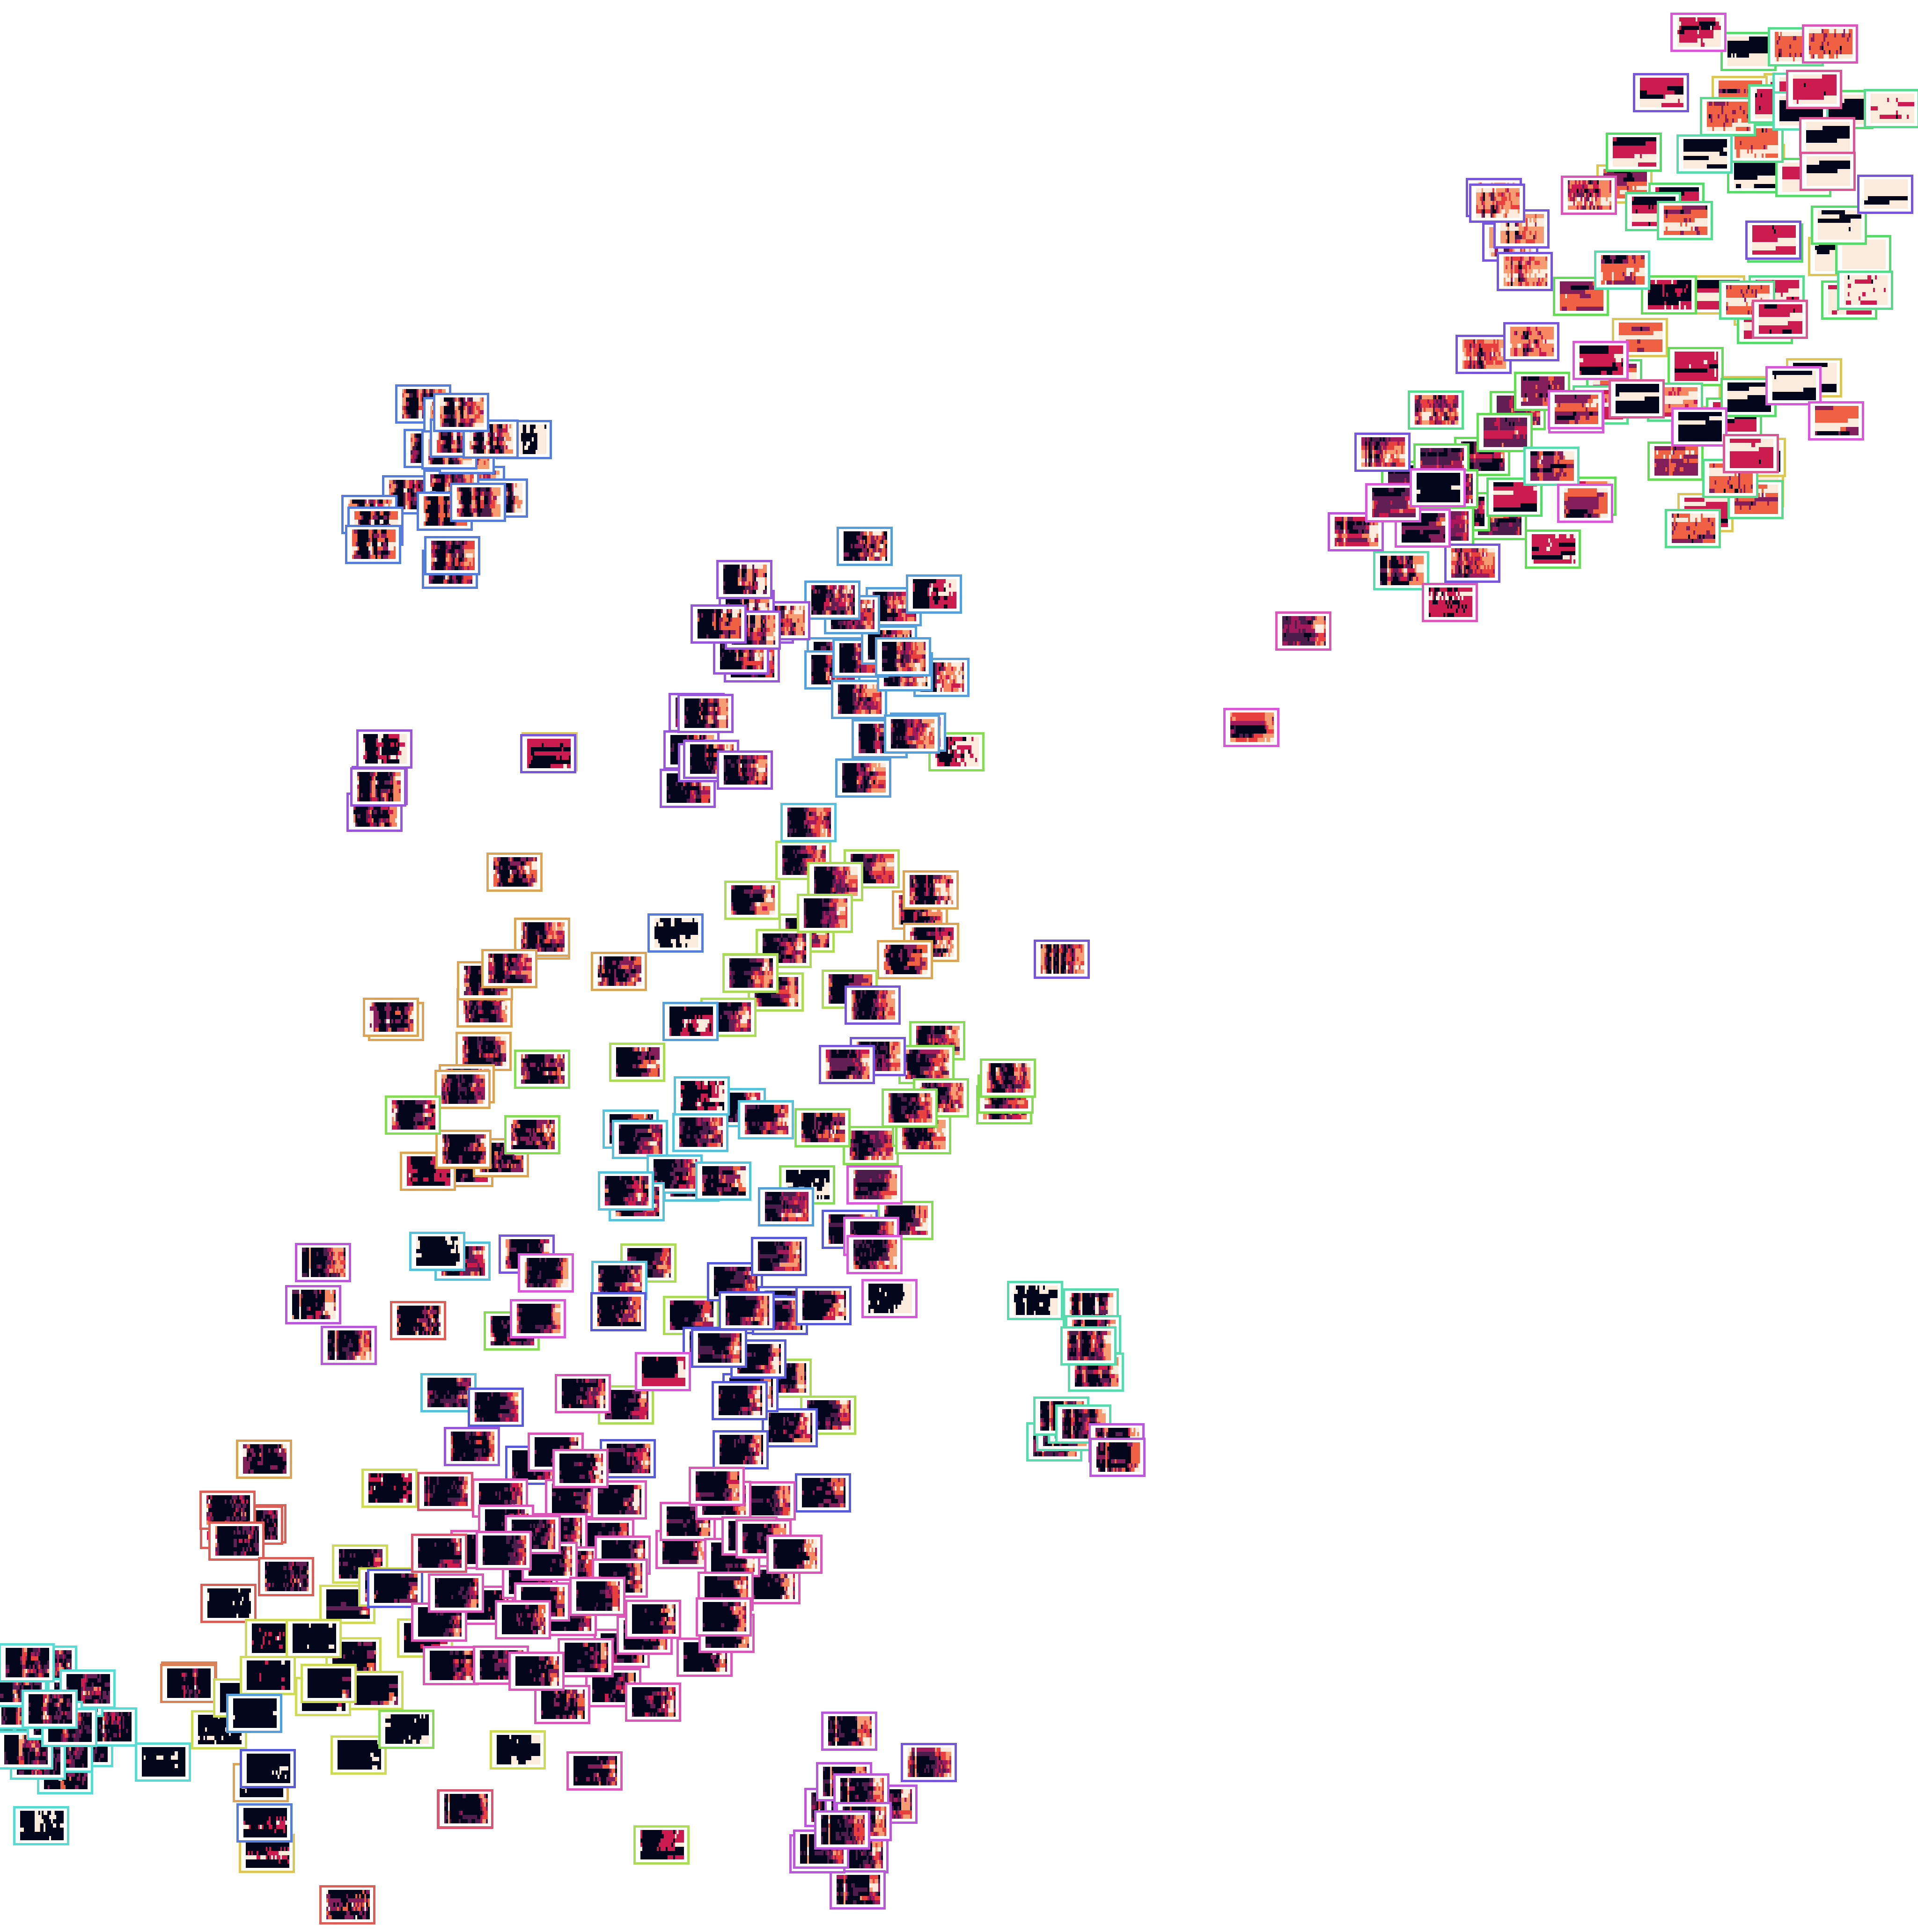
\includegraphics[width=.9\textwidth]{Figures/TSNE/TSNE_per_appliance/all/img_scatter_alltelevision.png}
	\label{fig:tsne_pa_img_scatter_all_tv}
\end{figure}

\subsubsection{Per-appliance load profiles - comparing appliances}

The figure \label{fig:tsne_papb_scatter_all} presents
the general picture of where each appliance lays in comparison to each other.
One obvious issue here is that there are too many appliances, and it is impossible to comprehend the plot.

\begin{figure}[H]
	\centering
	\caption{"Projection of per-appliance load profiles"}
	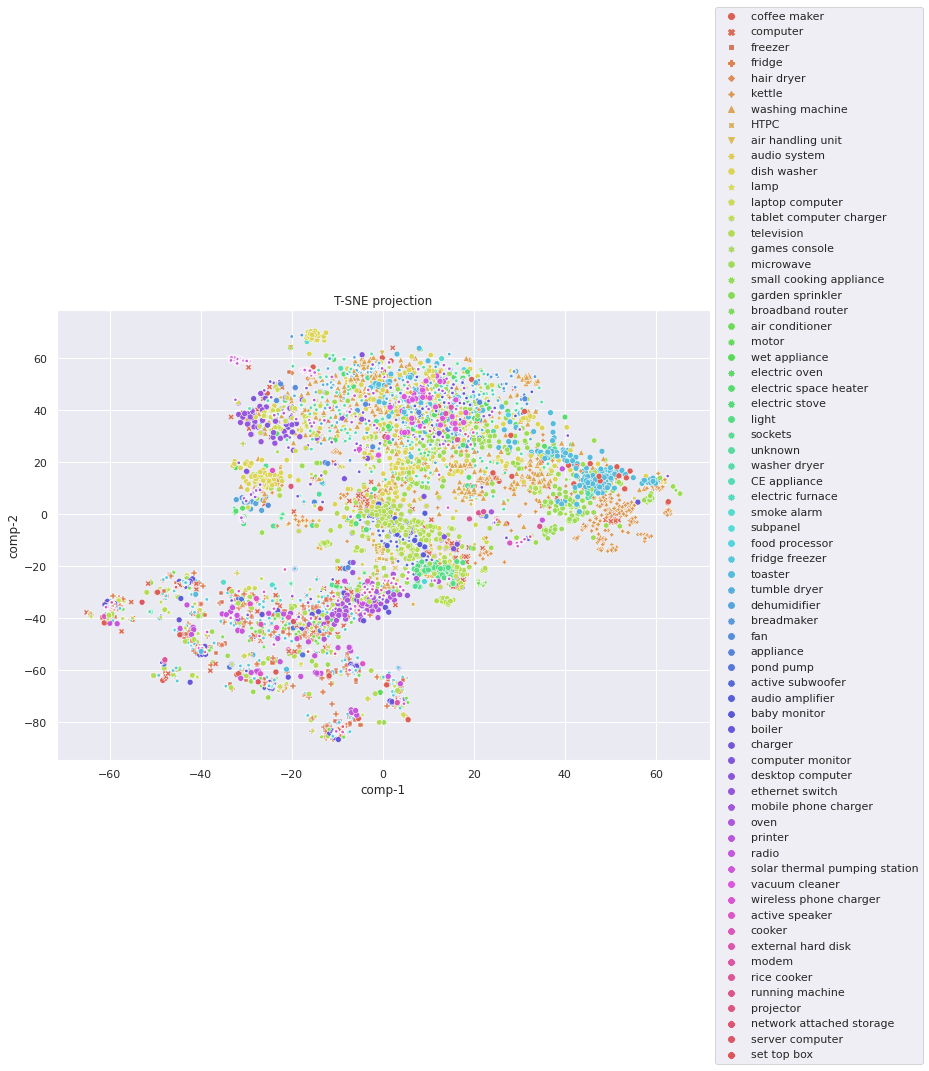
\includegraphics[width=1.2\textwidth]{Figures/TSNE/TSNE_results/all/scatter_all_all_lgimgs.png}
	\label{fig:tsne_papb_scatter_all}
\end{figure}

The same goes for image presentation on figure \ref{fig:tsne_papb_img_scatter_all}. 
We can see, that most active appliances are the ones in the bottom left,
by moving to the upper right part of the corer, we can see less activity.
Less activity does not necessarily mean that load profiles contain less information about user behavior.

\begin{figure}[H]
	\centering
	\caption{"Projection of per-appliance load profiles with actual samples"}
	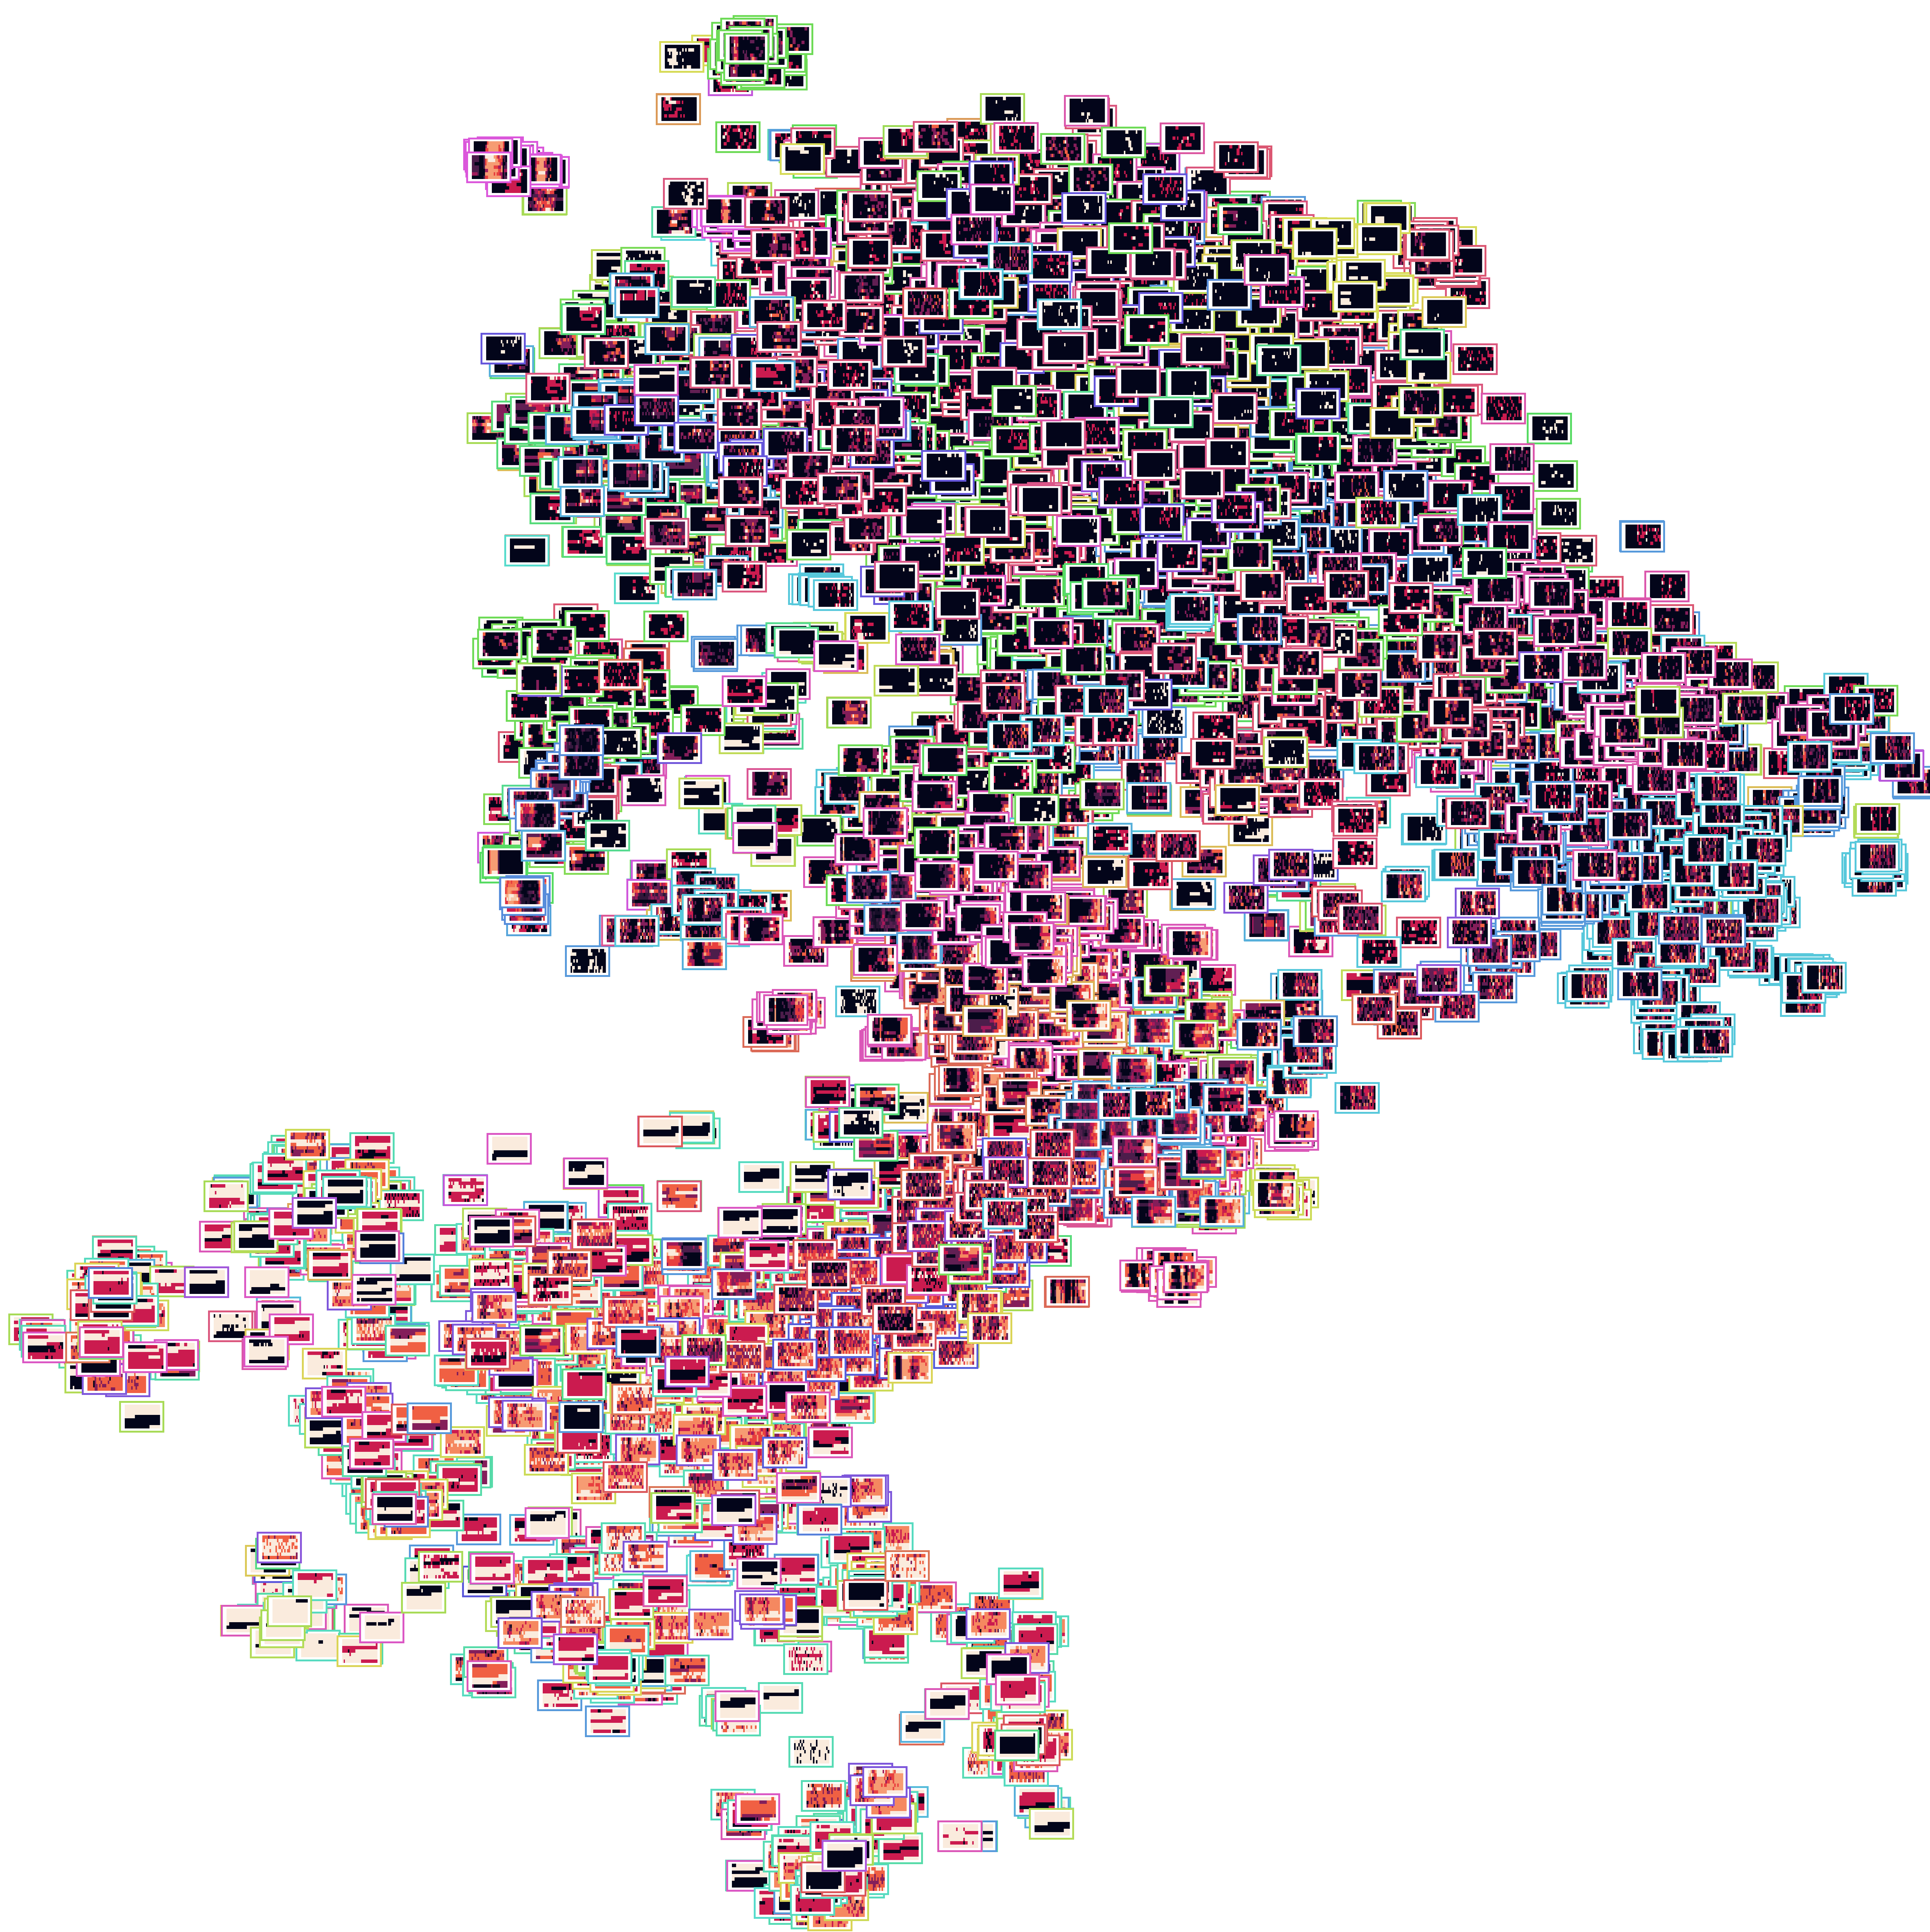
\includegraphics[width=.9\textwidth]{Figures/TSNE/TSNE_results/all/img_scatter_allall_lgimgs.png}
	\label{fig:tsne_papb_img_scatter_all}
\end{figure}

To get a general idea of where each appliance group lies,
let's filter out all appliances that have less than 150 samples.
Applying this filter yields figure \ref{fig:tsne_papb_scatter_all_reduced}.

\begin{figure}[H]
	\centering
	\caption{"Projection of filtered per-appliance load profiles"}
	\includegraphics[width=1.1\textwidth]{Figures/TSNE/TSNE_results/all/scatter_all_all_reduced_max.png}
	\label{fig:tsne_papb_scatter_all_reduced}
\end{figure}

The figure \ref{fig:tsne_papb_scatter_all_reduced} shows how these 10 appliances ares connected in high dimensional space.
Kettle, microwave and toaster are quite similar when it comes to usage patterns.
They are operated for a short amount of time and are usually used in users' routines in the morning or evening.
These appliances are located in the upper left part of the plot.

The second group of appliances that are quite near each other is white
goods (without fridges) such as washing machines, dishwashers, dryers etc.
Let's say that they are white goods with a program. 
This group of appliances is located in the upper right part of the plot.

The third group of appliances is white goods with a compressor.
They are usually not affected by human interaction and are therefore harder to cluster.
They are located in the lower part of the plot.

The final group of appliances is televisions and computers. They lie 
on a bridge between the fridges and other groups. 

\begin{figure}[H]
	\centering
	\caption{"Projection of filtered per-appliance load profiles with actual samples"}
	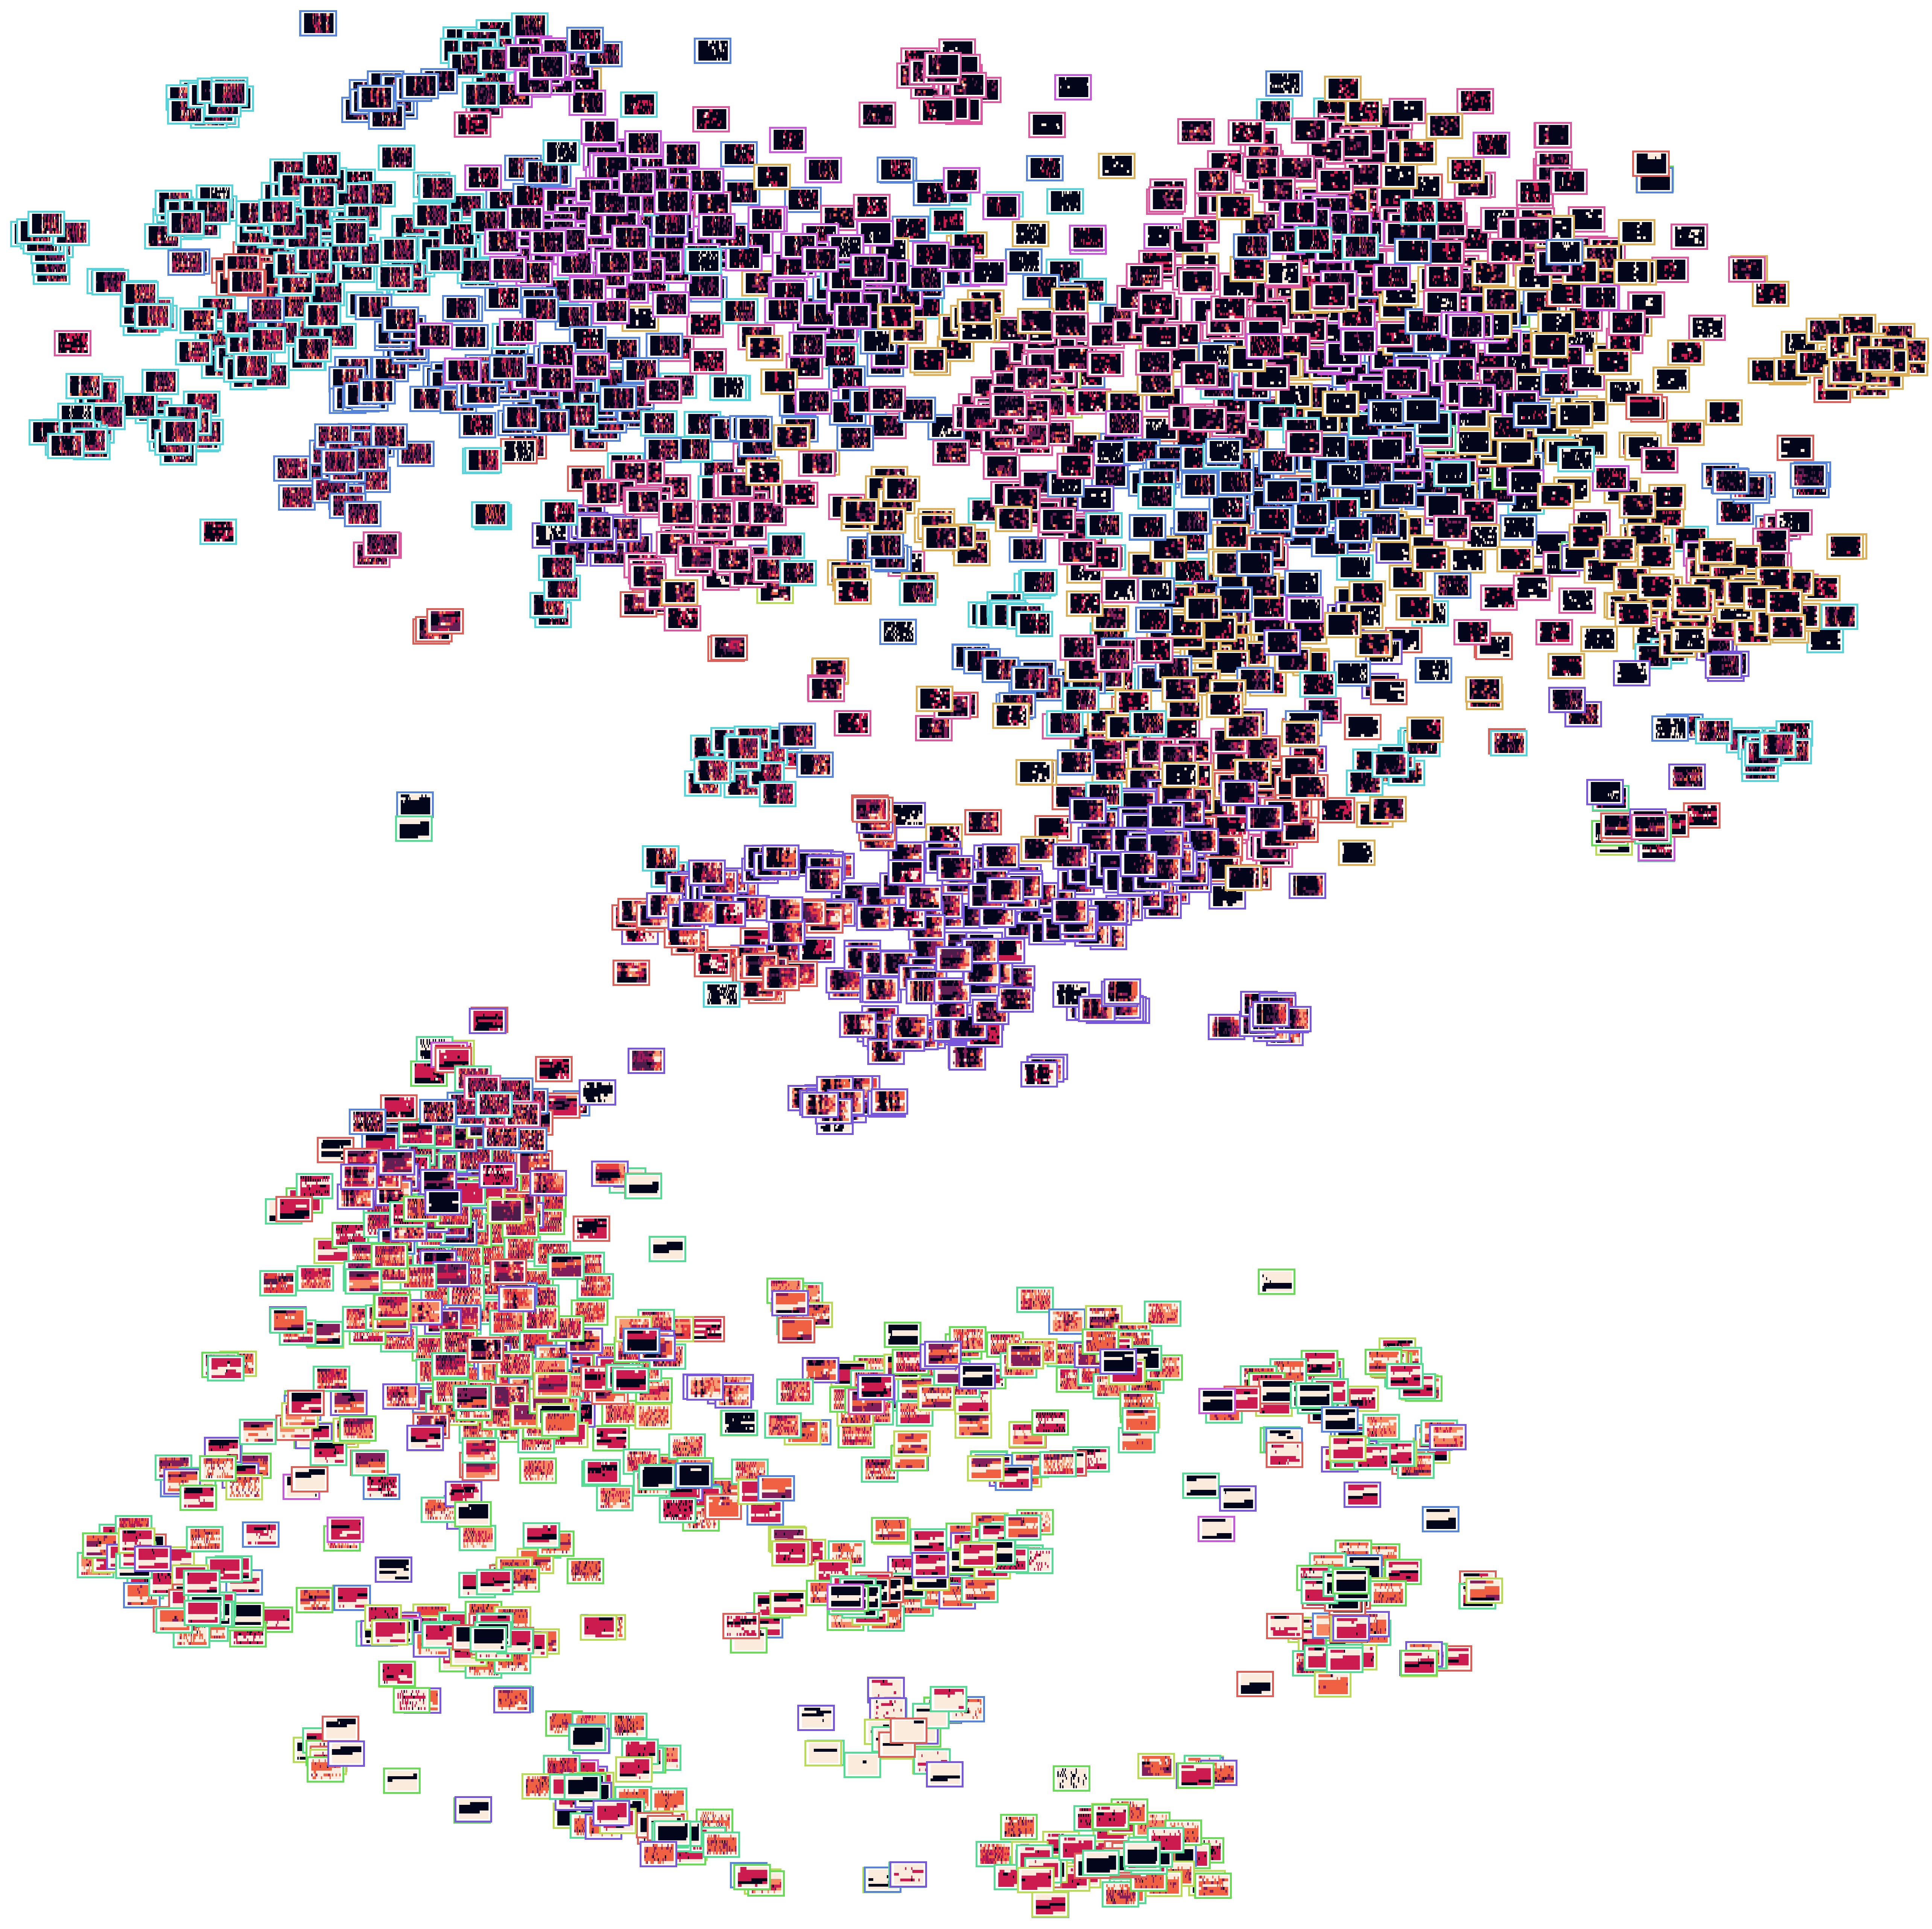
\includegraphics[width=.9\textwidth]{Figures/TSNE/TSNE_results/all/img_scatter_allall_reduced_max.png}
	\label{fig:tsne_papb_img_scatter_all_reduced}
\end{figure}

All through the set of load profiles is different due to filtering,
the figure \ref{fig:tsne_papb_img_scatter_all_reduced},
retains a similar structure to the previous figure \ref{fig:tsne_papb_scatter_all_reduced}. 

Knowing that a pattern exists, we can use the newly found group to define new appliance groups.
The following 8 groups will be defined
\begin{itemize}
    \item Kitchen appliances - toasters, ovens, microwaves, etc.
    \item Fridges and freezers  - contains fridges, freezers and fridge freezers or white goods with a compressor
    \item White goods - washers, dryers, dishwashers i.e. white goods with a program
    \item heating and cooling - Electric radiators, dehumidifiers and HVACs
    \item leisure -  Living room appliances such as TVs, games consoles, audio amps, HTPCs, etc.
    \item home office - Computer, laptops, printers, network equipment, chargers, etc.
    \item lightning - lights and lamps
    \item Others - unknown and unlabeled appliances
\end{itemize}

Applying these groups yields figure \ref{fig:tsne_papb_scatter_all_groups}.
The new plot shows how, although appliances could be used by a different
user, maybe even by users in a different part of the EU or world,
they can be grouped in a high-dimensional space. 

\begin{figure}[H]
	\centering
	\caption{"Projection of grouped per-appliance load profiles"}
	\includegraphics[width=.8\textwidth]{Figures/TSNE/TSNE_results/all/scatter_all_all_groups.png}
	\label{fig:tsne_papb_scatter_all_groups}
\end{figure}

The figure \ref{fig:tsne_papb_img_scatter_all_groups} below is the same as the first figure \ref{fig:tsne_papb_img_scatter_all} in the subsection,
except it is easier to use color to see the appliance they present

\begin{figure}[H]
	\centering
	\caption{"Projection of grouped per-appliance load profiles with actual samples"}
	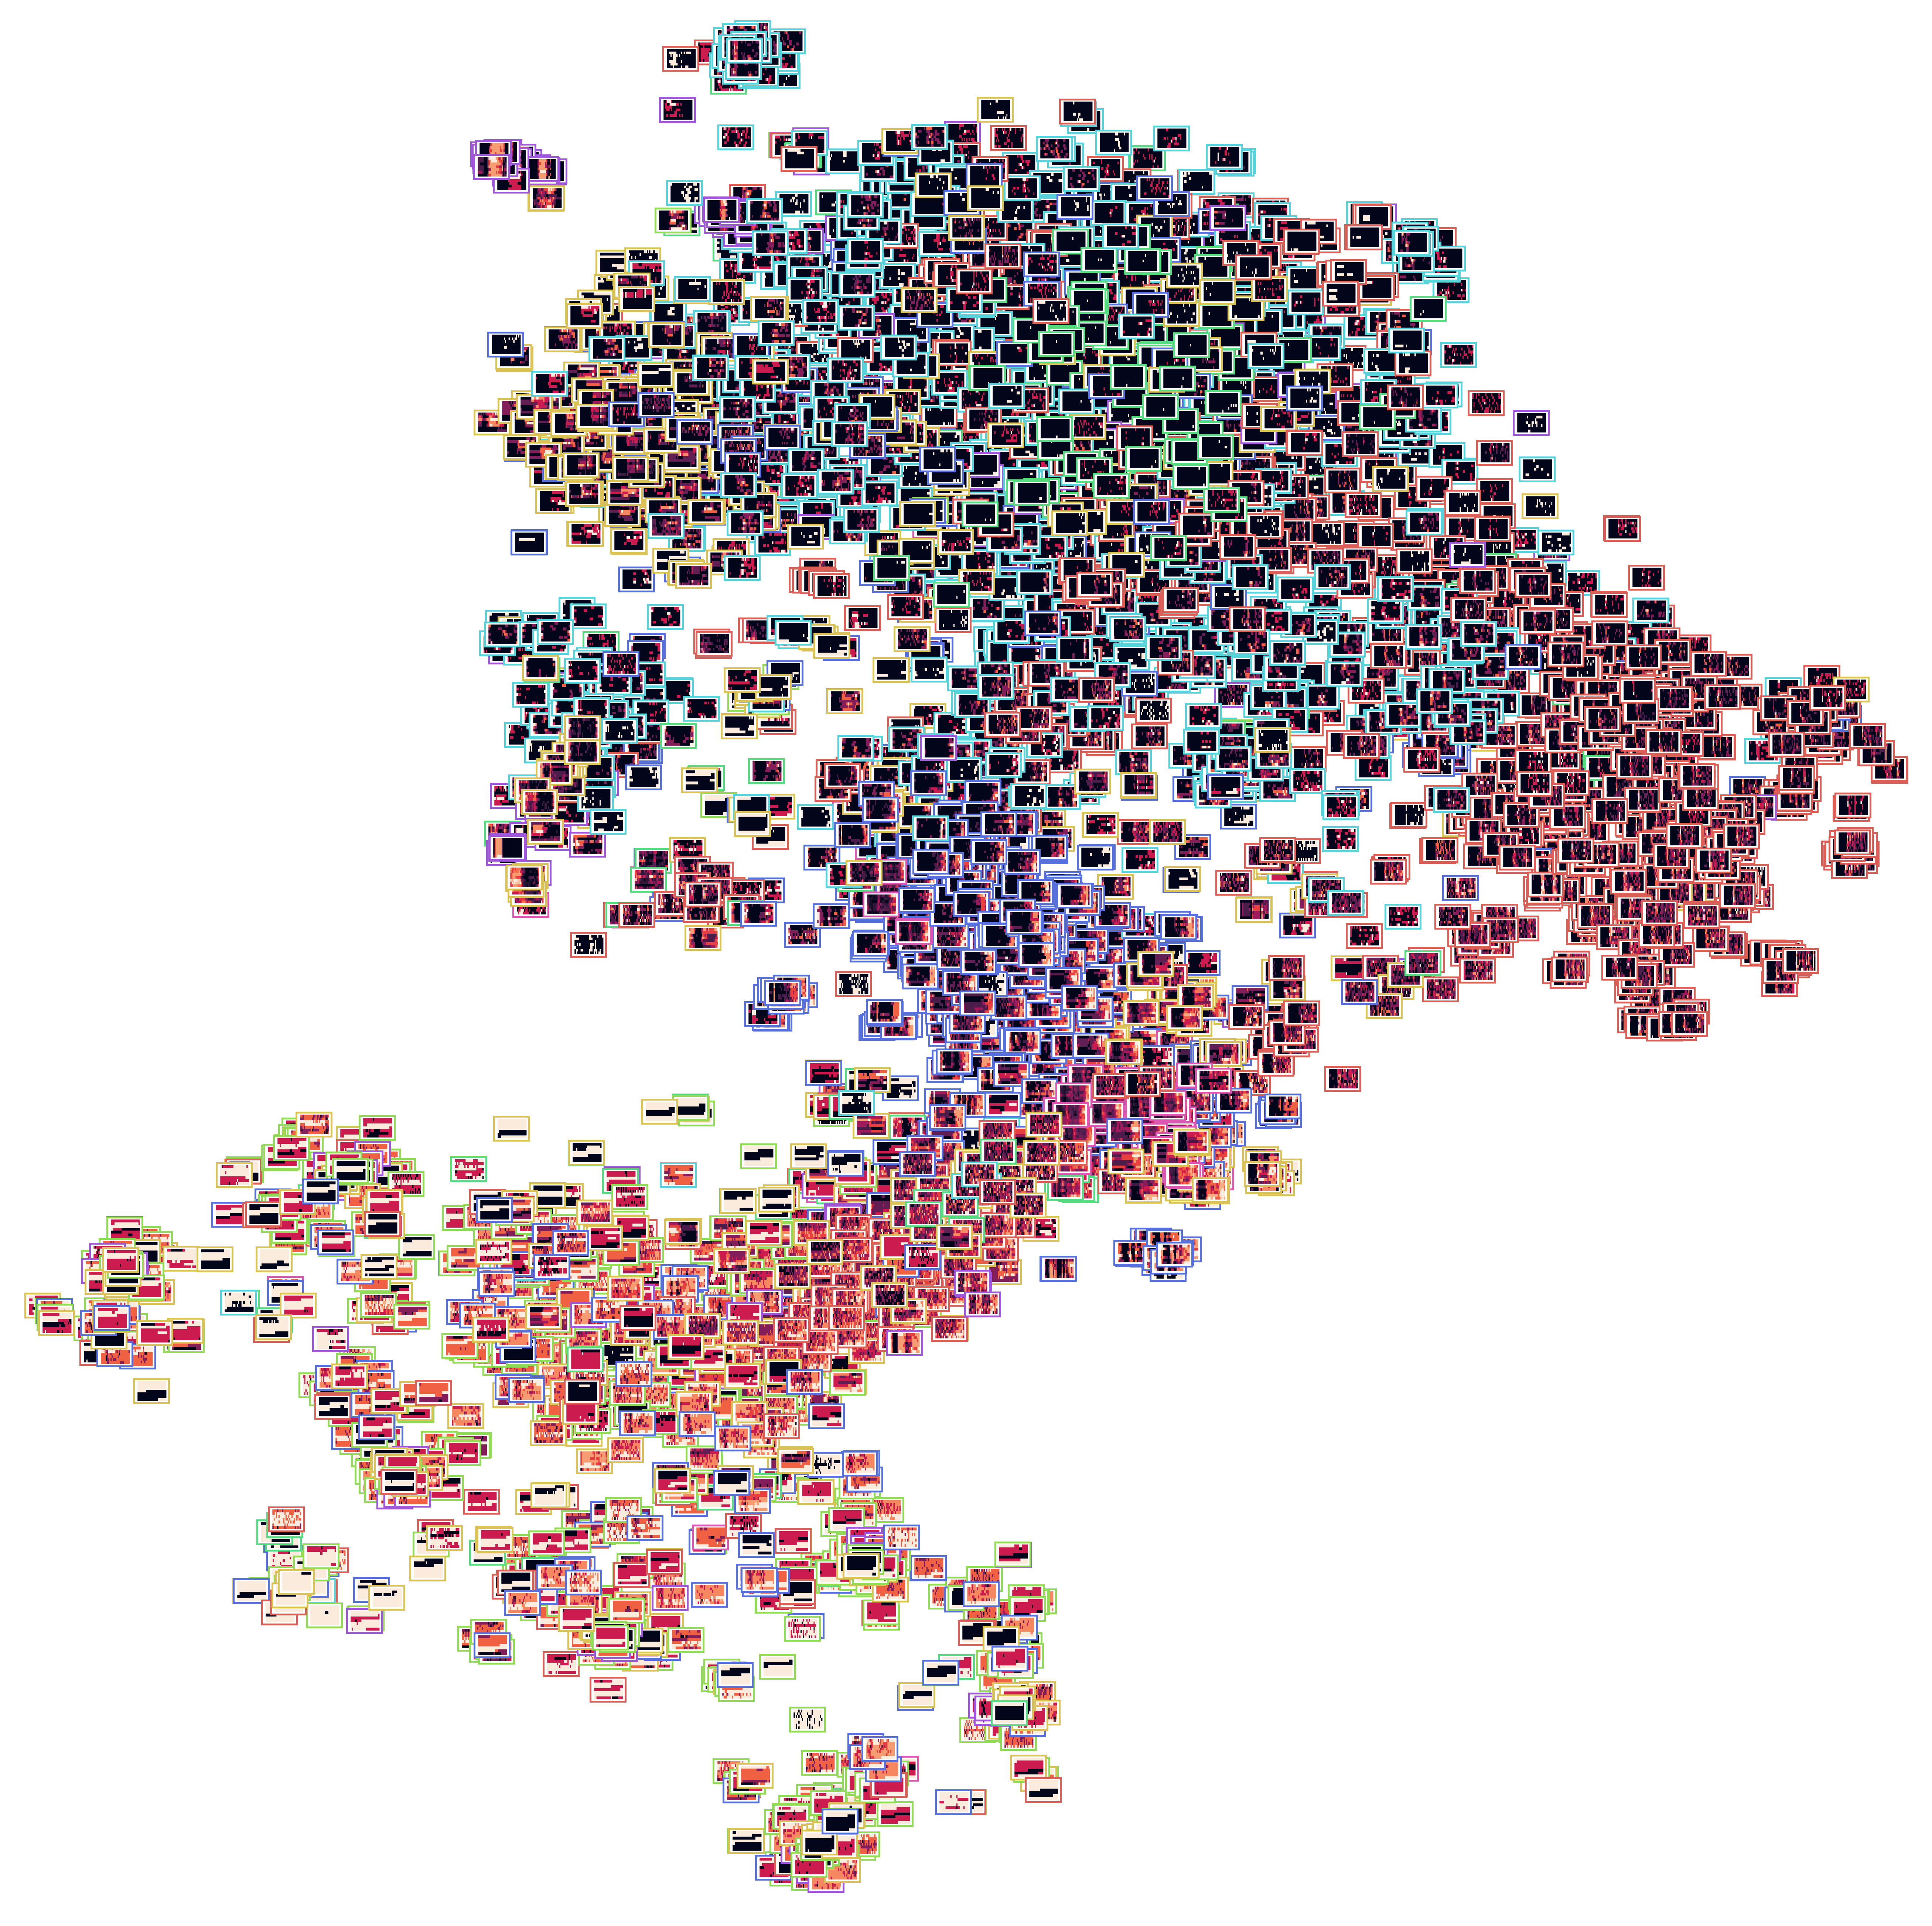
\includegraphics[width=.9\textwidth]{Figures/TSNE/TSNE_results/all/img_scatter_all_all_groups.png}
	\label{fig:tsne_papb_img_scatter_all_groups}
\end{figure}

The figure \ref{fig:t-sne_zoomed} shows the four main types of profiles for readers that do not have the ability to zoom in.

\begin{figure}[H]
	\centering
	\caption{"Projection of grouped per-appliance load profiles with actual samples"}
	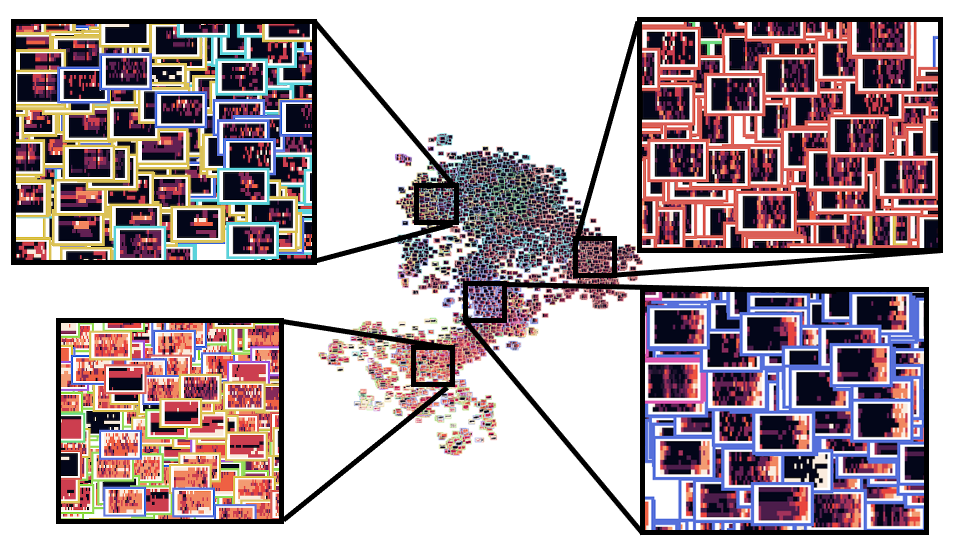
\includegraphics[width=.9\textwidth]{Figures/TSNE/TSNE_results/all/t-sne_zoomed.png}
	\label{fig:t-sne_zoomed}
\end{figure}

One issue that causes the t-SNE algorithm an issue is low entropy data or 
in other words, images that are almost completely dark or white, due to various faults in appliances or measurements.

If we calculate entropy for each image and set a threshold, it is possible to filter out these samples. 
By setting an entropy threshold of 0.5, we filter out around 5 \% of all samples. 

\begin{figure}[H]
	\centering
	\caption{"Projection of entropy filtered per-appliance load profiles"}
	\includegraphics[width=.8\textwidth]{Figures/TSNE/TSNE_results_entropy/all/scatter_all_all.png}
	\label{fig:tsne_papb_scatter_ent_all_groups}
\end{figure}

Again, we can apply appliance grouping and get nicely formed clusters, such as can be seen in figure \ref{fig:tsne_papb_img_scatter_ent_all_groups}.

\begin{figure}[H]
	\centering
	\caption{"Projection of entropy filtered per-appliance load profiles with actual samples"}
	\includegraphics[width=.8\textwidth]{Figures/TSNE/TSNE_results_entropy/all/scatter_all_all_groups.png}
	\label{fig:tsne_papb_img_scatter_ent_all_groups}
\end{figure}


\subsubsection{Comparing appliances in a building}

It is also possible to use per-appliance data to study
individual buildings, and how each appliance is used.
In this case, we have used building 8 from REFIT as an example.

\begin{figure}[H]
	\centering
	\caption{"Projection of per-appliance load profiles in a single building"}
	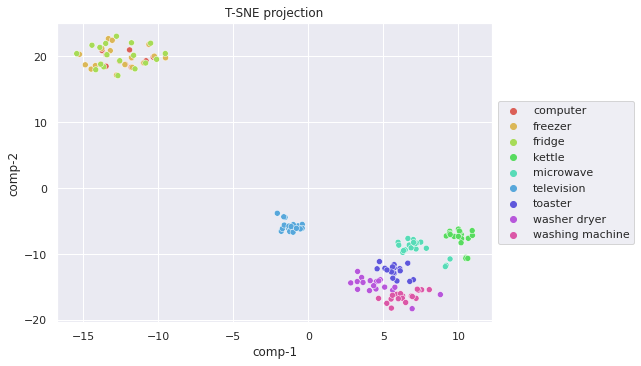
\includegraphics[width=.8\textwidth]{Figures/TSNE/TSNE_results/refit/scatter_refit_8.png}
	\label{fig:tsne_papb_scatter_ent_refit8}
\end{figure}

In general, the scattering is similar to before.
Fridge and freezers are located opposite of white goods and kitchen appliances and 
the television lies somewhere in between. 

\begin{figure}[H]
	\centering
	\caption{"Projection of per-appliance load profiles in a single building with actual samples"}
	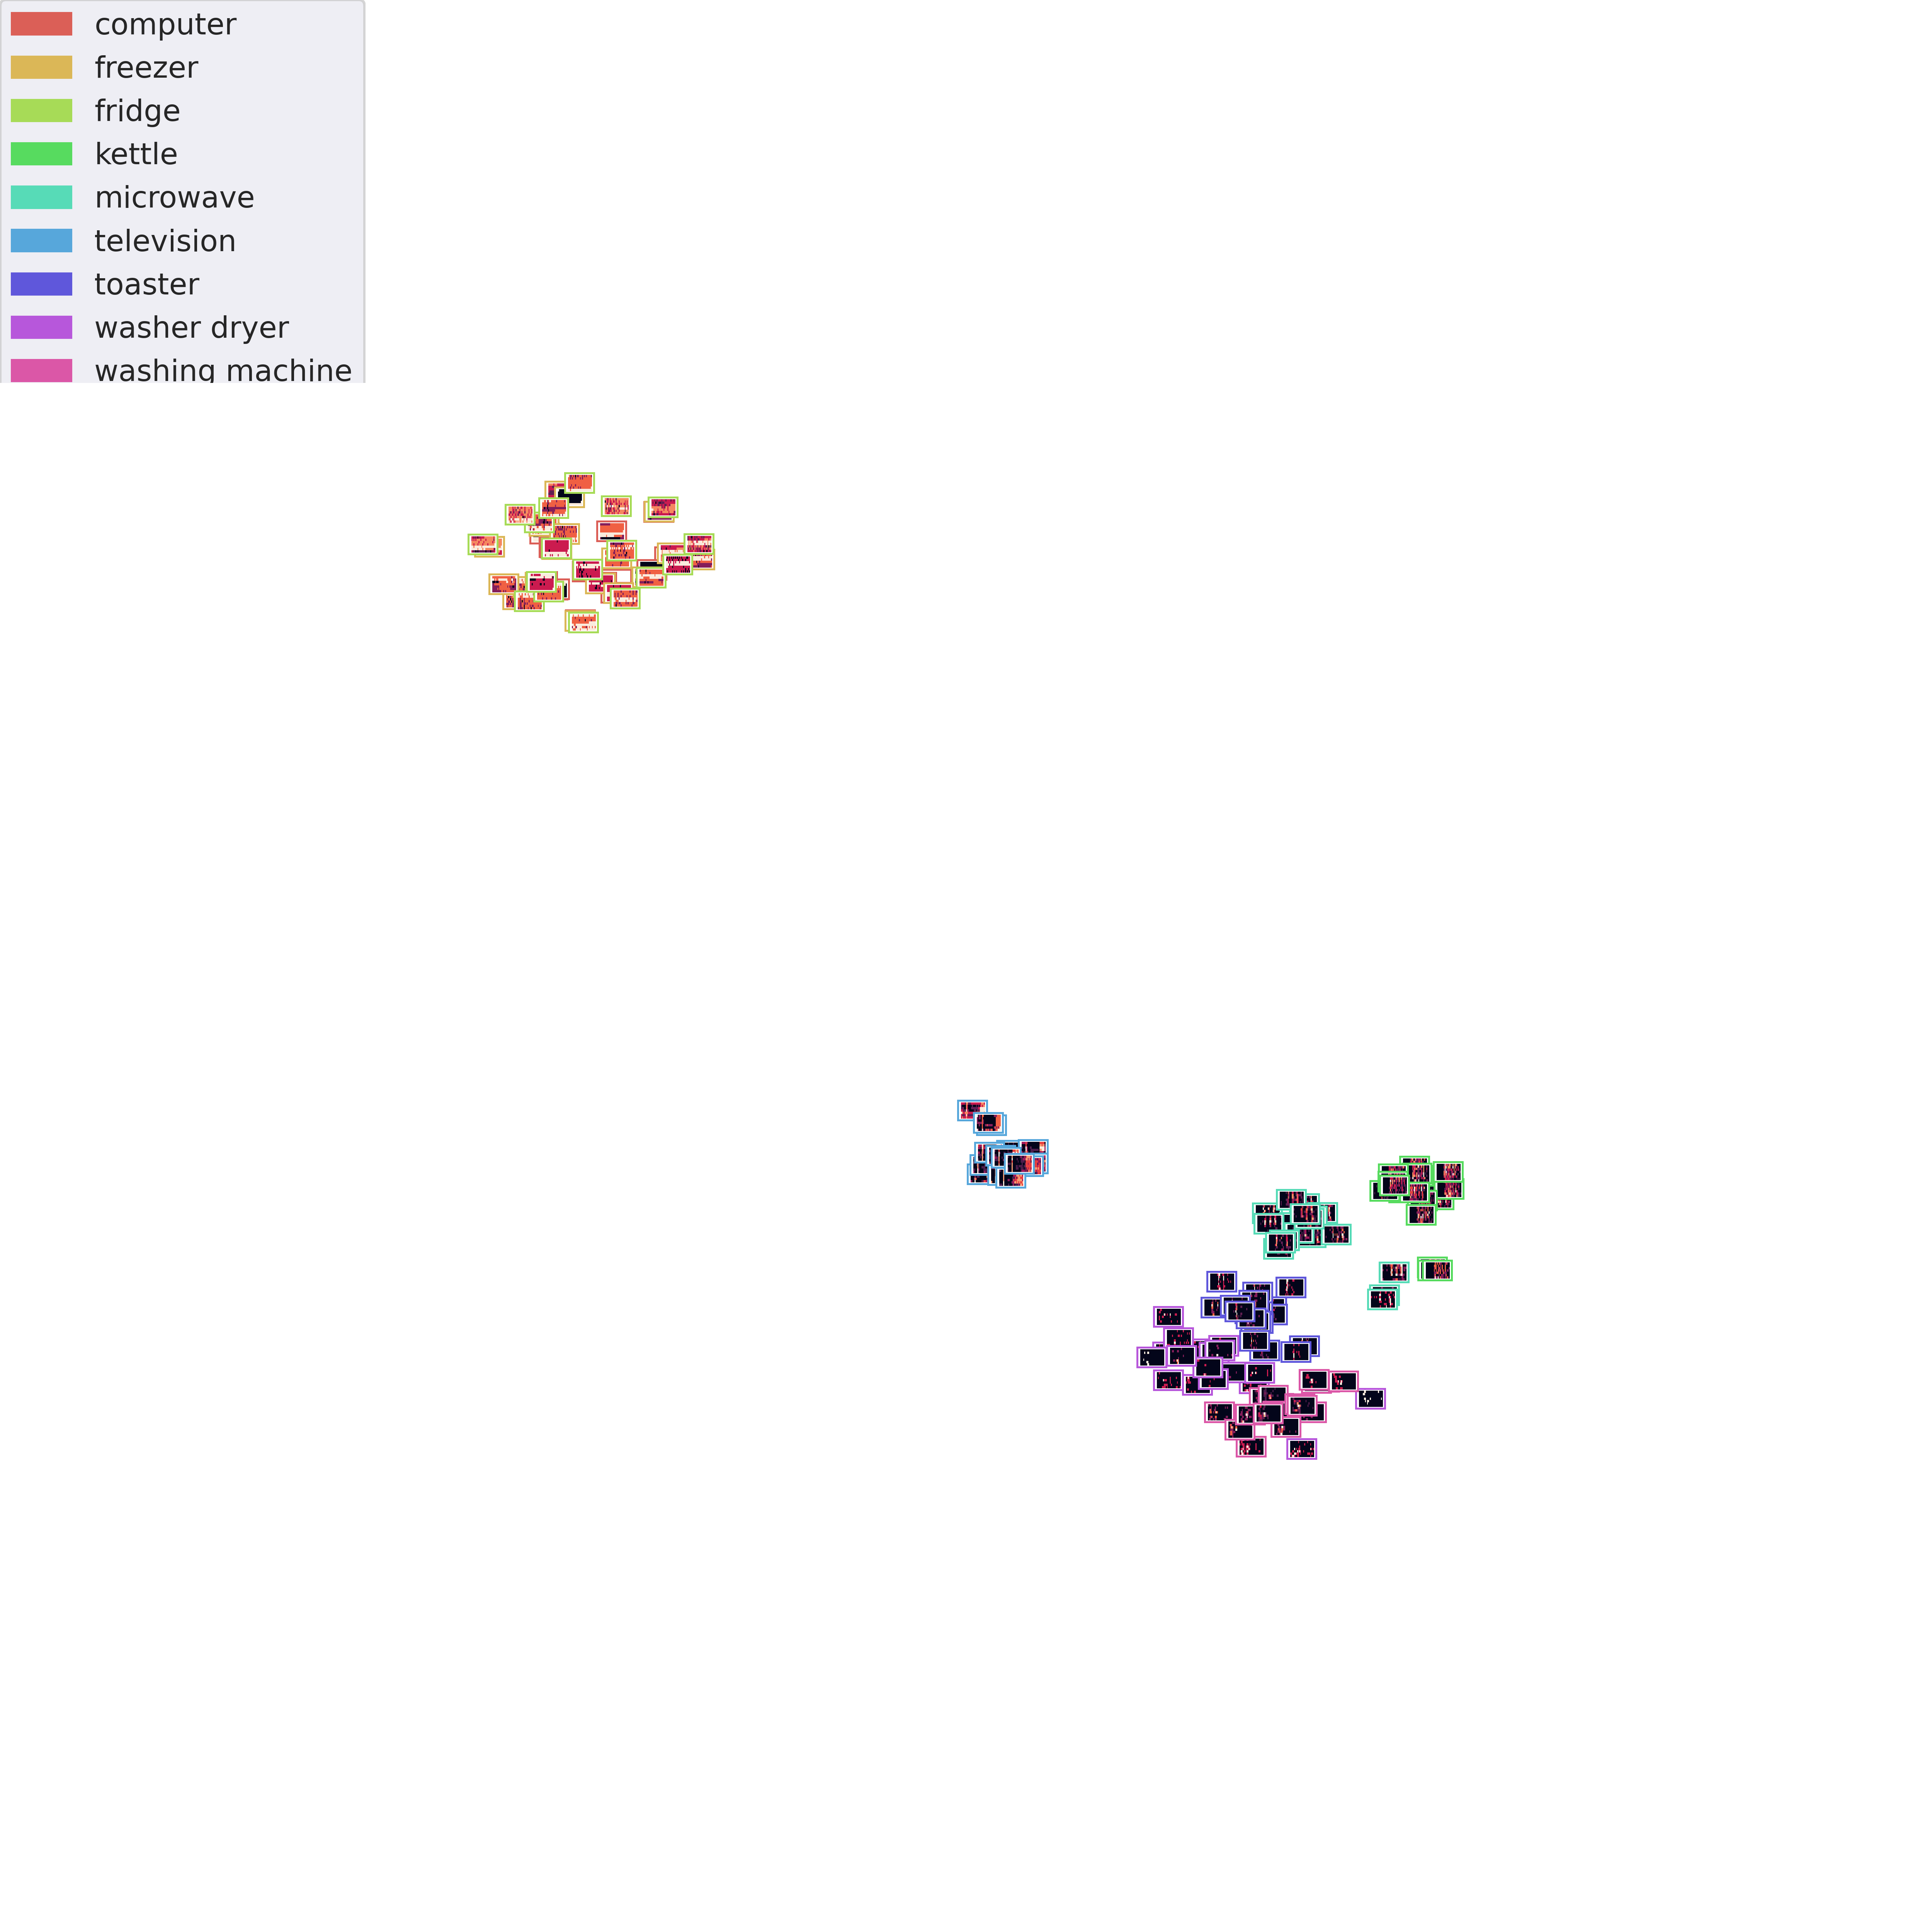
\includegraphics[width=.9\textwidth]{Figures/TSNE/TSNE_results/refit/img_scatter_refit8.png}
	\label{fig:tsne_papb_img_scatter_ent_refit8}
\end{figure}

Similar as before figure \label{fig:tsne_papb_img_scatter_ent_refit8} shows fridge cluster as the most active,
with the least interesting information. In the middle, we can again observe the TV that is mostly being used
in the evening hours. The samples also point to the possibility of a high user routine in the early morning hours.
The high routine is portrayed as a straight line on the figures. 

In this case, when observing white goods in ping and purple boxes, it is possible to see that this user primarily uses them during the night hours.
This could point out that the user is making use of cheaper tariffs.

One other interesting observation that can be made here is comparing kettles and microwaves and toasters.
Usually, these appliances are used similarly and in similar parts of the day. 
Here the toaster and microwave are being used periodically, but the kettle is being used throughout the day with no general pattern.
It is self-obvious that some users have higher routines than others, but this observation
would add that some users can have a higher routine for some appliances and lower for others. 

\subsection{Per-appliance per-building}

To study the usage by comparing all appliances between buildings,
we have to use one of the proposed load profiles and in this case, this is a Bag of appliances.

\subsubsection{Bag of appliances}
This load profile is a combination of the load profiles above,
except it offers a larger detail when observing groups of appliances.
Since we are using one dimension for appliances, we will use only the daily dimension.

To construct such a profile we need a universal way of constructing it.
This is done by measuring how many times each appliance occurs in the datasets,
then this list is sorted from most common to least common, and finally, the top 30 are selected.
The results are appliances in the following order:

The problem with such a comparison is, that it is best 
if all buildings would use the same appliance.
Since that is not the case, missing appliances are portrayed as always off. 

This is the main reason why we can see in figure \ref{fig:tsne_boa_scatter_refit8} the clusters are nicely formed
but are separated quite a lot. We can still see that some clusters are closer than others,
meaning they are more similar.

\begin{figure}[H]
	\centering
	\caption{"Projection of bag of appliances load profiles for various buildings"}
	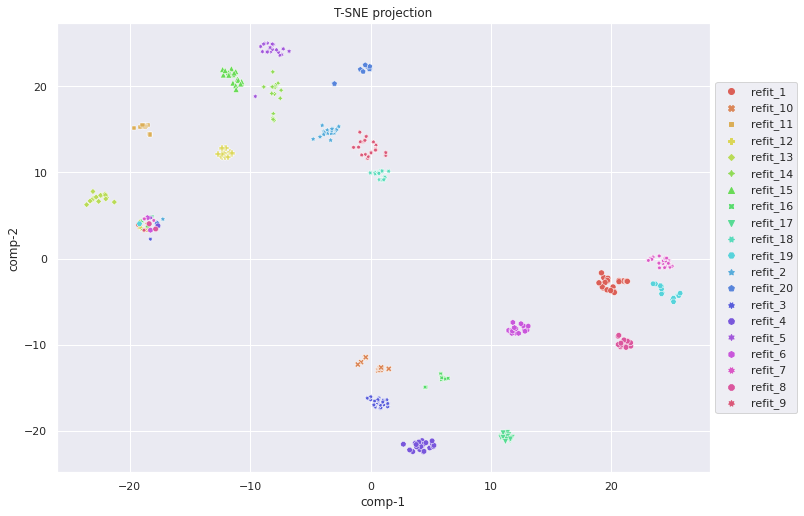
\includegraphics[width=.8\textwidth]{Figures/TSNE/TSNE_BOA/refit/scatter_refit_all.png}
	\label{fig:tsne_boa_scatter_refit8}
\end{figure}

Figure \ref{fig:tsne_boa_img_scatter_refit8} shows that load profiles are split 
between two poles. By observing the figure it is possible to see that the bottom Clusters
all have more than one active white good with a compressor (fridges and freezers), while
the top ones have only one. In general, the bottom buildings have more appliances,
with more activity than the top ones. 

\begin{figure}[H]
	\centering
	\caption{"Projection of bag of appliances load profiles for various buildings with actual samples"}
	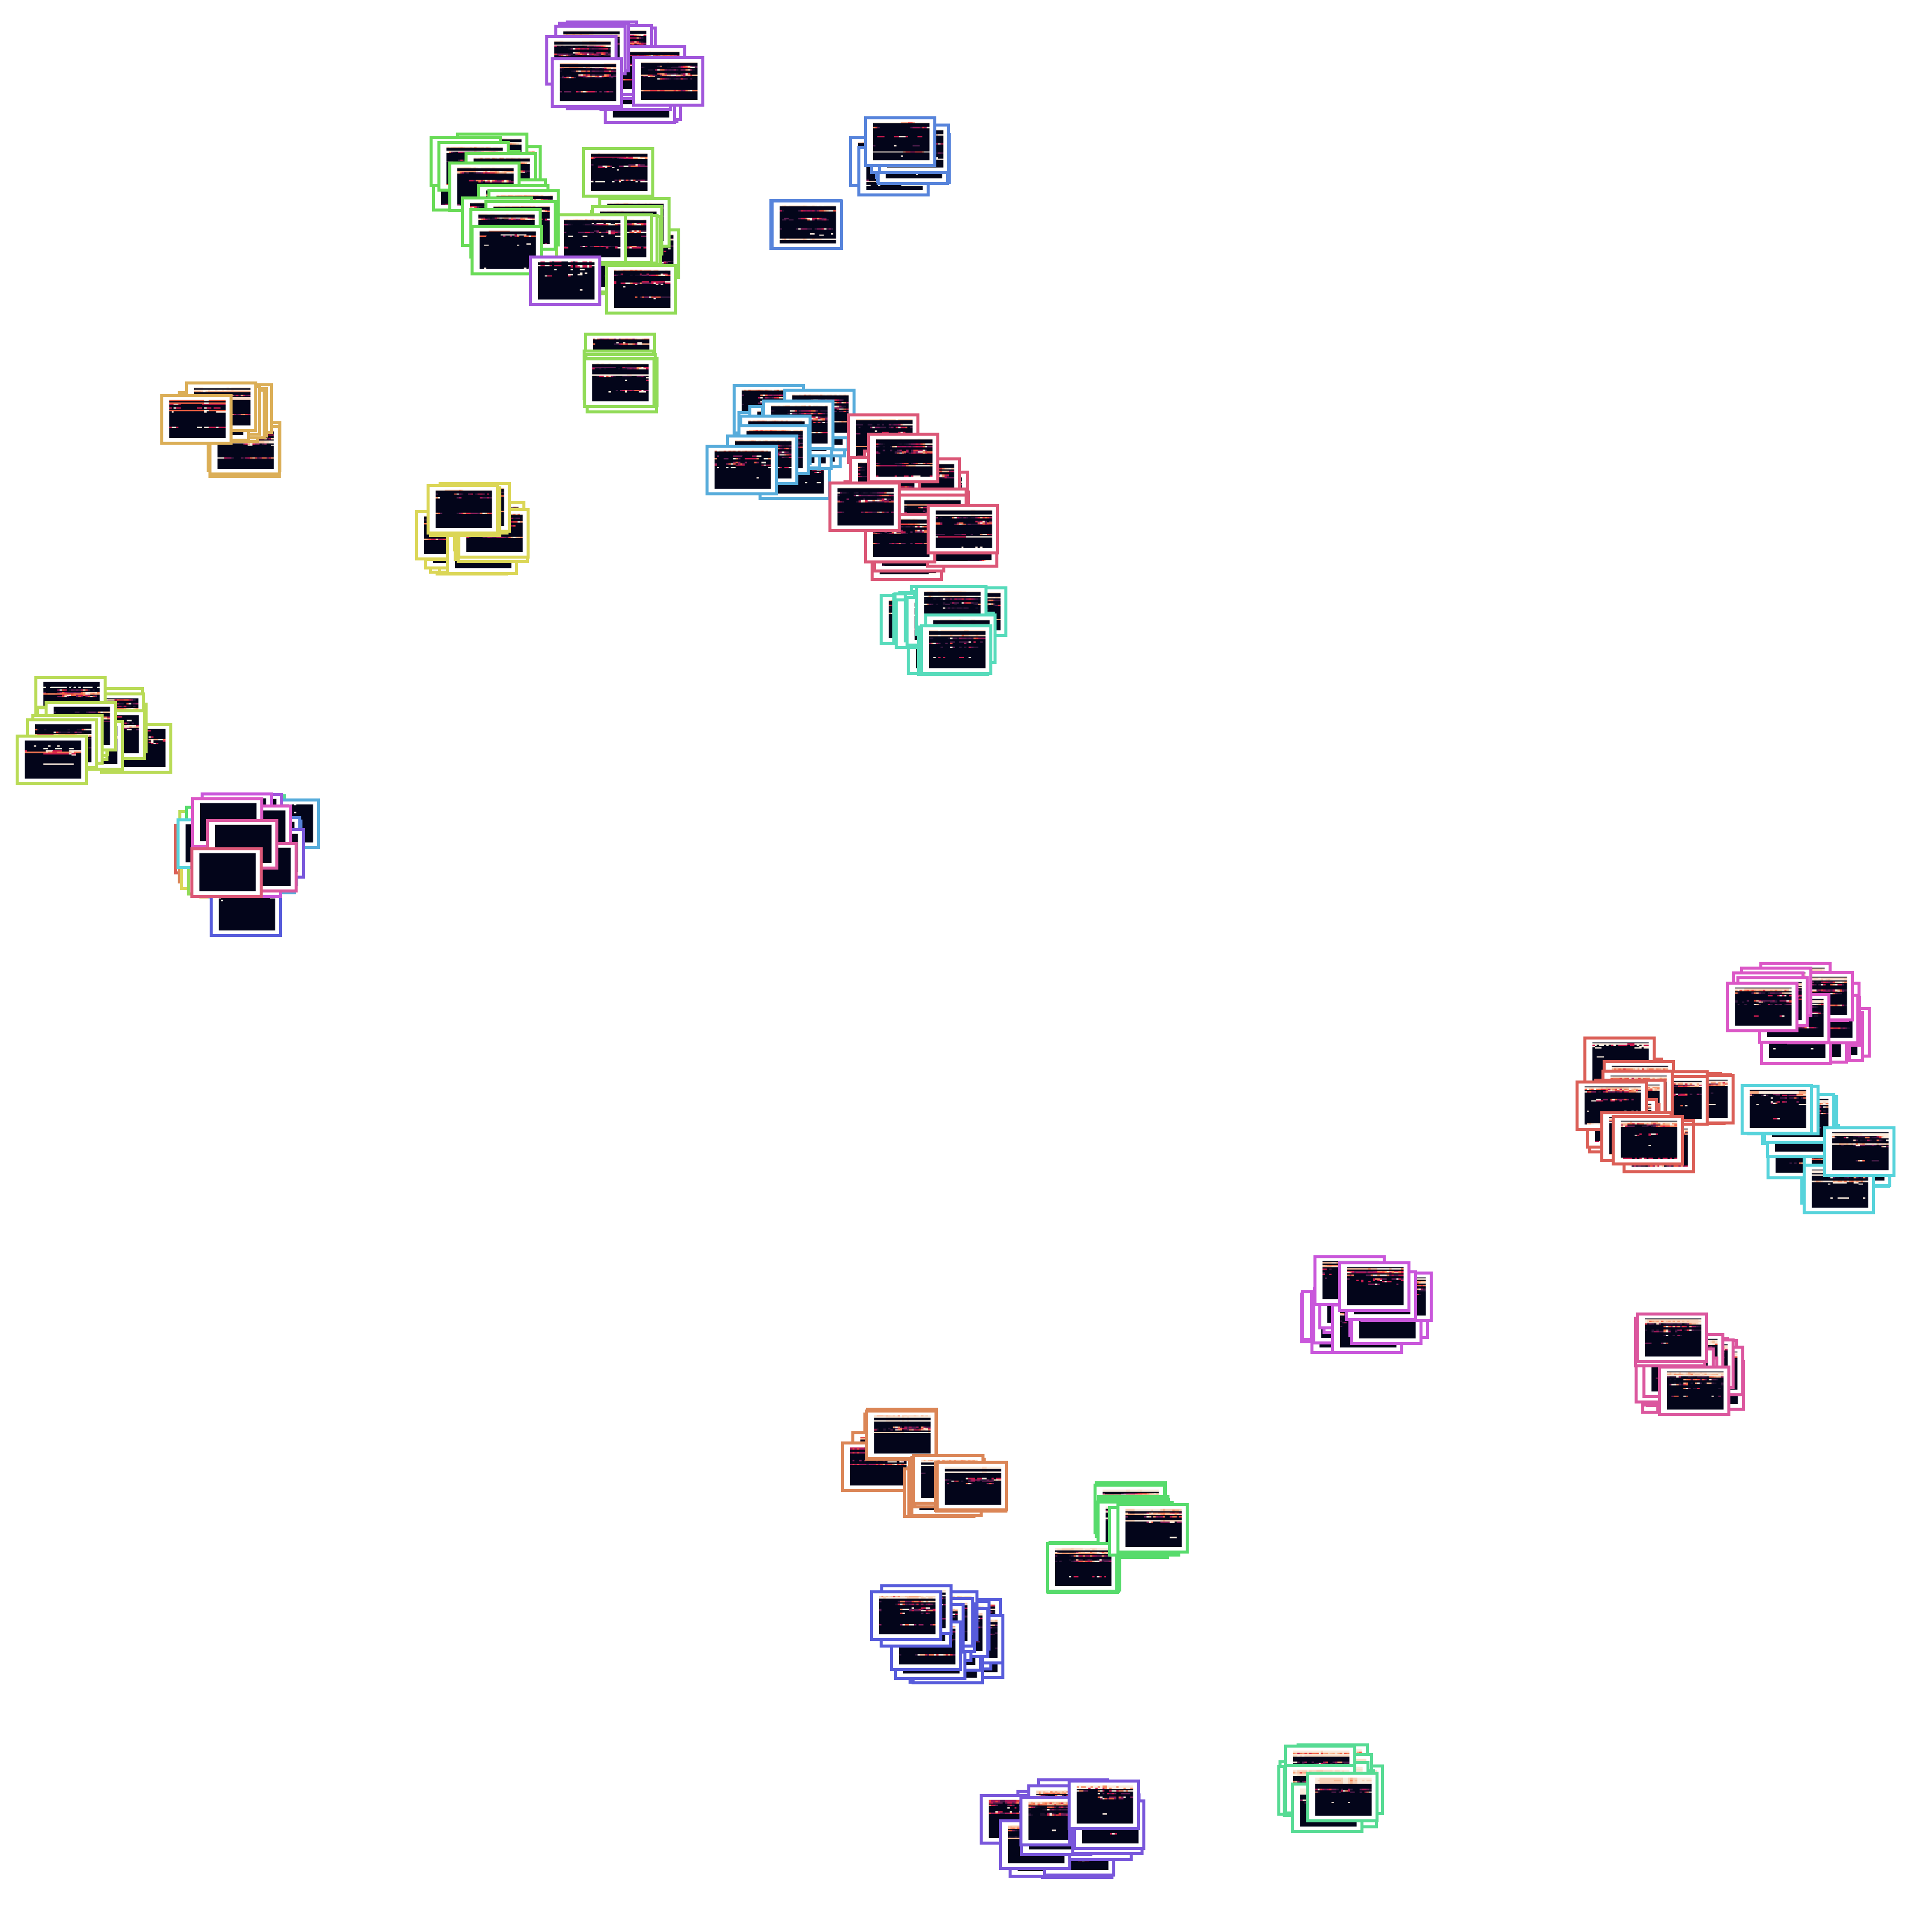
\includegraphics[width=.9\textwidth]{Figures/TSNE/TSNE_BOA/refit/img_scatter_refitall.png}
	\label{fig:tsne_boa_img_scatter_refit8}
\end{figure}

\section{Discussion}

The main goal of the chapter was to show how data is related in high-dimensional space.
For this to be achieved, three different types of load profiles were utilized. 

Per-building load profiles offered a look into how activations patterns differ across different buildings and datasets.
Per-building per-appliance bag of appliance load profiles offered the same thing, but in greater detail.
Per-appliance load profiles were the most versatile and were utilized in the most various ways.
First, we have shown how the same type of appliance is being used across various buildings.
Next, we have compared appliances between each other. 
Since the plot was incomplete, we have defined appliance groups.
These new groups formed clusters, which revealed the connection between types of profiles. 
Finally, we compared how appliances in a single building. 

\section{Conclusion}

We have seen how samples and samples are connected and related in higher dimensions, this should enable us to be more efficient when using these load profiles in the next chapter. 
The comprehensive analysis of the plots pointed out that we can roughly estimate the strength of a routine based on the scattering of load profiles.
This information will be useful in the next chapter where we will utilize it to build the elderly care system.

While there are no empirical results to present, the effect of seeing the actual samples placed on a map was stronger.
We could go into greater detail and use other dimensionality-reduction algorithms for comparison, but that was not the goal.
The side goal, besides the main one, was to show and present the patterns in the data and other features such as a routine strength.
While doing that we also proved that the load profiles that we proposed can be efficiently used to do that.

Knowing this we can conclude the chapter by stating that we have successfully utilized previously unused load profiles, and thus made a scientific contribution.
